\documentclass[a4paper,USenglish,cleveref,autoref,thm-restate]{lipics-v2021}
%This is a template for producing LIPIcs articles. 
%See lipics-v2021-authors-guidelines.pdf for further information.
%for A4 paper format use option "a4paper", for US-letter use option "letterpaper"
%for british hyphenation rules use option "UKenglish", for american hyphenation rules use option "USenglish"
%for section-numbered lemmas etc., use "numberwithinsect"
%for enabling cleveref support, use "cleveref"
%for enabling autoref support, use "autoref"
%for anonymousing the authors (e.g. for double-blind review), add "anonymous"
%for enabling thm-restate support, use "thm-restate"
%for enabling a two-column layout for the author/affilation part (only applicable for > 6 authors), use "authorcolumns"
%for producing a PDF according the PDF/A standard, add "pdfa"

\pdfoutput=1 %uncomment to ensure pdflatex processing (mandatatory e.g. to submit to arXiv)
\hideLIPIcs  %uncomment to remove references to LIPIcs series (logo, DOI, ...), e.g. when preparing a pre-final version to be uploaded to arXiv or another public repository

%\graphicspath{{./graphics/}}%helpful if your graphic files are in another directory

\nolinenumbers

\bibliographystyle{plainurl}% the mandatory bibstyle

\title{A Program Logic for Under-approximating Worst-case Resource Usage} %TODO Please add

%\titlerunning{Dummy short title} %TODO optional, please use if title is longer than one line

\author{Ziyue Jin}{Peking University}{zyjin@stu.pku.edu.cn}{}{}
\author{Di Wang}{Peking University}{wangdi95@pku.edu.cn}{}{}

\authorrunning{Z. Jin and D. Wang}

%\author{Jane {Open Access}}{Dummy University Computing Laboratory, [optional: Address], Country \and My second affiliation, Country \and \url{http://www.myhomepage.edu} }{johnqpublic@dummyuni.org}{https://orcid.org/0000-0002-1825-0097}{(Optional) author-specific funding acknowledgements}%TODO mandatory, please use full name; only 1 author per \author macro; first two parameters are mandatory, other parameters can be empty. Please provide at least the name of the affiliation and the country. The full address is optional. Use additional curly braces to indicate the correct name splitting when the last name consists of multiple name parts.

%\author{Joan R. Public\footnote{Optional footnote, e.g. to mark corresponding author}}{Department of Informatics, Dummy College, [optional: Address], Country}{joanrpublic@dummycollege.org}{[orcid]}{[funding]}

%\authorrunning{J. Open Access and J.\,R. Public} %TODO mandatory. First: Use abbreviated first/middle names. Second (only in severe cases): Use first author plus 'et al.'

%\Copyright{Jane Open Access and Joan R. Public} %TODO mandatory, please use full first names. LIPIcs license is "CC-BY";  http://creativecommons.org/licenses/by/3.0/

\begin{CCSXML}
<ccs2012>
<concept>
<concept_id>10003752.10003790.10003806</concept_id>
<concept_desc>Theory of computation~Programming logic</concept_desc>
<concept_significance>500</concept_significance>
</concept>
</ccs2012>
\end{CCSXML}

\ccsdesc[500]{Theory of computation~Programming logic}
%TODO mandatory: Please choose ACM 2012 classifications from https://dl.acm.org/ccs/ccs_flat.cfm 

\keywords{Under-approximation, Incorrectness logic, Worst-case Resource Bounds} %TODO mandatory; please add comma-separated list of keywords

%\category{} %optional, e.g. invited paper

%\relatedversion{} %optional, e.g. full version hosted on arXiv, HAL, or other respository/website
%\relatedversiondetails[linktext={opt. text shown instead of the URL}, cite=DBLP:books/mk/GrayR93]{Classification (e.g. Full Version, Extended Version, Previous Version}{URL to related version} %linktext and cite are optional

%\supplement{}%optional, e.g. related research data, source code, ... hosted on a repository like zenodo, figshare, GitHub, ...
%\supplementdetails[linktext={opt. text shown instead of the URL}, cite=DBLP:books/mk/GrayR93, subcategory={Description, Subcategory}, swhid={Software Heritage Identifier}]{General Classification (e.g. Software, Dataset, Model, ...)}{URL to related version} %linktext, cite, and subcategory are optional

%\funding{(Optional) general funding statement \dots}%optional, to capture a funding statement, which applies to all authors. Please enter author specific funding statements as fifth argument of the \author macro.

%\acknowledgements{I want to thank \dots}%optional

%\nolinenumbers %uncomment to disable line numbering



%Editor-only macros:: begin (do not touch as author)%%%%%%%%%%%%%%%%%%%%%%%%%%%%%%%%%%
%\EventEditors{John Q. Open and Joan R. Access}
%\EventNoEds{2}
%\EventLongTitle{42nd Conference on Very Important Topics (CVIT 2016)}
%\EventShortTitle{CVIT 2016}
%\EventAcronym{CVIT}
%\EventYear{2016}
%\EventDate{December 24--27, 2016}
%\EventLocation{Little Whinging, United Kingdom}
%\EventLogo{}
%\SeriesVolume{42}
%\ArticleNo{23}
%%%%%%%%%%%%%%%%%%%%%%%%%%%%%%%%%%%%%%%%%%%%%%%%%%%%%%

\usepackage{amsmath}
\usepackage{mathpartir}
\usepackage{mathtools}
\usepackage{dsfont}
\usepackage{xcolor}
\usepackage{MnSymbol}
\usepackage{graphicx}
\usepackage{stmaryrd}
\usepackage{anyfontsize}
\usepackage{algorithm}
\usepackage{algpseudocode}
\usepackage{shortcuts}
\usepackage{cleveref}
\usepackage{booktabs}
\crefname{theorem}{Thm.}{Thms.}
\crefname{lemma}{Lem.}{Lemmas}
\crefname{corollary}{Cor.}{Cors.}
\crefname{figure}{Fig.}{Figs.}
\crefname{definition}{Defn.}{Defns.}
\crefname{table}{Tab.}{Tabs.}
\crefformat{section}{\S#2#1#3}
\crefmultiformat{section}{\S#2#1#3}{ and~\S#2#1#3}{, \S#2#1#3}{ and~\S#2#1#3}
\crefname{example}{Ex.}{Exs.}
\crefname{item}{item}{items}
\crefname{footnote}{footnote}{footnotes}
\crefname{observation}{Obs.}{Obs.}
\crefname{remark}{Remark}{Remarks}
\crefname{proposition}{Prop.}{Props.}
\crefname{equation}{Eqn.}{Eqns.}
\crefname{counterexample}{Counterexample}{Counterexamples}
\crefname{property}{Property}{Properties}
\crefname{algorithm}{Algorithm}{Algorithms}
\usepackage{subcaption}

\newcommand{\Blue}[1]{\textcolor{blue}{#1}}
\newcommand{\Red}[1]{\textcolor{red}{#1}}
\newcommand{\Gray}[1]{\textcolor{gray}{#1}}

\renewcommand{\dagger}{\text{\textdagger}}

\newcommand{\QBUAd}{QBUA\textsuperscript{$\Diamond$}\ }
\newcommand{\Bd}{B\textsuperscript{$\Diamond$}}

\newcommand{\pjudge}[3]{\vdash\left\{#1\right\}#2\left\{#3\right\}}

\newcommand{\Judge}[3]{\vDash\left[#1\right]#2\left[#3\right]}
\newcommand{\judge}[3]{\vdash\left[#1\right]#2\left[#3\right]}

\newcommand{\bjudge}[3]{\vdash_{\mathsf{B}}\left[#1\right]#2\left[#3\right]}
\newcommand{\fjudge}[3]{\vdash_{\mathsf{F}}\left[#1\right]#2\left[#3\right]}
\newcommand{\ajudge}[3]{\vdash_{\dagger}\left[#1\right]#2\left[#3\right]}
\newcommand{\djudge}[3]{\vdash^{\Diamond}_{\mathsf{B}}\left[#1\right]#2\left[#3\right]}
\newcommand{\bJudge}[3]{\vDash_{\mathsf{B}}\left[#1\right]#2\left[#3\right]}
\newcommand{\fJudge}[3]{\vDash_{\mathsf{F}}\left[#1\right]#2\left[#3\right]}
\newcommand{\dJudge}[3]{\vDash^{\Diamond}_{\mathsf{B}}\left[#1\right]#2\left[#3\right]}

\newcommand{\bbjudge}[5]{\vdash_{\mathsf{B}}\left[\left.#1\right|#2\right]#3\left[\left.#4\right|#5\right]}
\newcommand{\ffjudge}[5]{\vdash_{\mathsf{F}}\left[\left.#1\right|#2\right]#3\left[\left.#4\right|#5\right]}
\newcommand{\aajudge}[5]{\vdash_{\dagger}\left[\left.#1\right|#2\right]#3\left[\left.#4\right|#5\right]}
\newcommand{\ddjudge}[5]{\vdash^{\Diamond}_{\mathsf{B}}\left[\left.#1\right|#2\right]#3\left[\left.#4\right|#5\right]}
\newcommand{\AAjudge}[5]{\vdash_{\text{\textdaggerdbl}}\left[\left.#1\right|#2\right]#3\left[\left.#4\right|#5\right]}

\newcommand{\bigstep}[6]{\left\langle#1,#2,#3\right\rangle\Downarrow^{#4}\left\langle#5,#6\right\rangle}
\newcommand{\bigstepp}[5]{\left\langle#1,#2,#3\right\rangle\Downarrow\left\langle#4,#5\right\rangle}
\newcommand{\bigstepl}[5]{\left\langle#1,#2,#3\right\rangle\Downarrow^{\le 0}\left\langle#4,#5\right\rangle}

\newcommand{\eval}[2]{\left\llbracket#1\right\rrbracket#2}

\newcommand{\post}[2]{\mathrm{post}\left\llbracket#1\right\rrbracket\left(#2\right)}
\newcommand{\pre}[2]{\mathrm{pre}\left\llbracket#1\right\rrbracket\left(#2\right)}
\newcommand{\prel}[2]{\mathrm{pre}^{\le 0}\left\llbracket#1\right\rrbracket\left(#2\right)}

\newcommand{\Skip}{\textsf{skip}}
\newcommand{\Assign}[2]{#1\coloneqq#2}
\newcommand{\Assume}[1]{\textsf{assume}~#1}
\newcommand{\Tick}[1]{\textsf{tick}~#1}
\newcommand{\Seq}[2]{#1;#2}
\newcommand{\Choice}[2]{#1+#2}
\renewcommand{\Loop}[1]{#1^*}
\newcommand{\Ite}[3]{\textsf{if}~#1~\textsf{then}~#2~\textsf{else}~#3}
\newcommand{\IfB}[1]{\textsf{if}~#1~\textsf{then}}
\renewcommand{\Else}{\textsf{else}}
\renewcommand{\While}[2]{\textsf{while}~#1~\textsf{do}~#2}
\newcommand{\WhileB}[1]{\textsf{while}~#1~\textsf{do}}
\newcommand{\Local}[2]{\textsf{local}~#1~\textsf{in}~#2}
\newcommand{\Localx}[1]{\textsf{local}~#1~\textsf{in}}

\newcommand{\SR}[2]{\left[\left.#1\right|#2\right]} %Spec and Resource

\newcommand{\Fv}{\mathrm{fv}}
\newcommand{\Mod}{\mathrm{mod}}

\newcommand{\Rinf}{\mathbb{R}^{\pm\infty}}
\newcommand{\Sup}{\mathop{\scalebox{-1}[1]{\textsf{S}}}}
\newcommand{\Inf}{\mathop{\scalebox{-1}[1]{\textsf{J}}}}

\newcommand{\true}{\mathsf{true}}
\newcommand{\false}{\mathsf{false}}

\newcommand{\Null}{\mathsf{null}}
\newcommand{\Val}{\mathsf{val}}
\newcommand{\Next}{\mathsf{next}}
\newcommand{\Lson}{\mathsf{lchild}}
\newcommand{\Rson}{\mathsf{rchild}}

\newcommand{\Time}[1]{#1_{\mathrm{time}}}

\algdef{SE}[SUBALG]{Indent}{EndIndent}{}{\algorithmicend\ }%
\algtext*{Indent}
\algtext*{EndIndent}

\sloppy

\begin{document}

\maketitle

%TODO mandatory: add short abstract of the document
\begin{abstract}
% State the problem
% Say why it's an interesting problem
% Say what your solution achieves
% Say what follows from your solution
%
Understanding and predicting the worst-case resource usage is crucial for software quality; however, existing methods either over-approximate with potentially loose bounds or under-approximate without asymptotic guarantees.
%
This paper presents a program logic to under-approximate worst-case resource usage, adapting incorrectness logic (IL) to reason quantitatively about resource consumption.
%
We propose \underline{q}uantitative \underline{f}orward and \underline{b}ackward \underline{u}nder-\underline{a}pproximate (QFUA and QBUA) triples, which generalize IL to identify execution paths leading to high resource usage.
%
We also introduce a variant of QBUA that supports reasoning about high-water marks.
%
Our logic is proven sound and complete with respect to a simple IMP-like language, and we demonstrate its utility through case studies involving arrays, pointers, and procedure calls.
%
%This work offers a formal, compositional framework for deriving lower bounds on resource usage, allowing for the identification of performance bottlenecks and security vulnerabilities in programs.
\end{abstract}

\section{Introduction}


\begin{figure}[t]
\centering
\includegraphics[width=0.6\columnwidth]{figures/evaluation_desiderata_V5.pdf}
\vspace{-0.5cm}
\caption{\systemName is a platform for conducting realistic evaluations of code LLMs, collecting human preferences of coding models with real users, real tasks, and in realistic environments, aimed at addressing the limitations of existing evaluations.
}
\label{fig:motivation}
\end{figure}

\begin{figure*}[t]
\centering
\includegraphics[width=\textwidth]{figures/system_design_v2.png}
\caption{We introduce \systemName, a VSCode extension to collect human preferences of code directly in a developer's IDE. \systemName enables developers to use code completions from various models. The system comprises a) the interface in the user's IDE which presents paired completions to users (left), b) a sampling strategy that picks model pairs to reduce latency (right, top), and c) a prompting scheme that allows diverse LLMs to perform code completions with high fidelity.
Users can select between the top completion (green box) using \texttt{tab} or the bottom completion (blue box) using \texttt{shift+tab}.}
\label{fig:overview}
\end{figure*}

As model capabilities improve, large language models (LLMs) are increasingly integrated into user environments and workflows.
For example, software developers code with AI in integrated developer environments (IDEs)~\citep{peng2023impact}, doctors rely on notes generated through ambient listening~\citep{oberst2024science}, and lawyers consider case evidence identified by electronic discovery systems~\citep{yang2024beyond}.
Increasing deployment of models in productivity tools demands evaluation that more closely reflects real-world circumstances~\citep{hutchinson2022evaluation, saxon2024benchmarks, kapoor2024ai}.
While newer benchmarks and live platforms incorporate human feedback to capture real-world usage, they almost exclusively focus on evaluating LLMs in chat conversations~\citep{zheng2023judging,dubois2023alpacafarm,chiang2024chatbot, kirk2024the}.
Model evaluation must move beyond chat-based interactions and into specialized user environments.



 

In this work, we focus on evaluating LLM-based coding assistants. 
Despite the popularity of these tools---millions of developers use Github Copilot~\citep{Copilot}---existing
evaluations of the coding capabilities of new models exhibit multiple limitations (Figure~\ref{fig:motivation}, bottom).
Traditional ML benchmarks evaluate LLM capabilities by measuring how well a model can complete static, interview-style coding tasks~\citep{chen2021evaluating,austin2021program,jain2024livecodebench, white2024livebench} and lack \emph{real users}. 
User studies recruit real users to evaluate the effectiveness of LLMs as coding assistants, but are often limited to simple programming tasks as opposed to \emph{real tasks}~\citep{vaithilingam2022expectation,ross2023programmer, mozannar2024realhumaneval}.
Recent efforts to collect human feedback such as Chatbot Arena~\citep{chiang2024chatbot} are still removed from a \emph{realistic environment}, resulting in users and data that deviate from typical software development processes.
We introduce \systemName to address these limitations (Figure~\ref{fig:motivation}, top), and we describe our three main contributions below.


\textbf{We deploy \systemName in-the-wild to collect human preferences on code.} 
\systemName is a Visual Studio Code extension, collecting preferences directly in a developer's IDE within their actual workflow (Figure~\ref{fig:overview}).
\systemName provides developers with code completions, akin to the type of support provided by Github Copilot~\citep{Copilot}. 
Over the past 3 months, \systemName has served over~\completions suggestions from 10 state-of-the-art LLMs, 
gathering \sampleCount~votes from \userCount~users.
To collect user preferences,
\systemName presents a novel interface that shows users paired code completions from two different LLMs, which are determined based on a sampling strategy that aims to 
mitigate latency while preserving coverage across model comparisons.
Additionally, we devise a prompting scheme that allows a diverse set of models to perform code completions with high fidelity.
See Section~\ref{sec:system} and Section~\ref{sec:deployment} for details about system design and deployment respectively.



\textbf{We construct a leaderboard of user preferences and find notable differences from existing static benchmarks and human preference leaderboards.}
In general, we observe that smaller models seem to overperform in static benchmarks compared to our leaderboard, while performance among larger models is mixed (Section~\ref{sec:leaderboard_calculation}).
We attribute these differences to the fact that \systemName is exposed to users and tasks that differ drastically from code evaluations in the past. 
Our data spans 103 programming languages and 24 natural languages as well as a variety of real-world applications and code structures, while static benchmarks tend to focus on a specific programming and natural language and task (e.g. coding competition problems).
Additionally, while all of \systemName interactions contain code contexts and the majority involve infilling tasks, a much smaller fraction of Chatbot Arena's coding tasks contain code context, with infilling tasks appearing even more rarely. 
We analyze our data in depth in Section~\ref{subsec:comparison}.



\textbf{We derive new insights into user preferences of code by analyzing \systemName's diverse and distinct data distribution.}
We compare user preferences across different stratifications of input data (e.g., common versus rare languages) and observe which affect observed preferences most (Section~\ref{sec:analysis}).
For example, while user preferences stay relatively consistent across various programming languages, they differ drastically between different task categories (e.g. frontend/backend versus algorithm design).
We also observe variations in user preference due to different features related to code structure 
(e.g., context length and completion patterns).
We open-source \systemName and release a curated subset of code contexts.
Altogether, our results highlight the necessity of model evaluation in realistic and domain-specific settings.





\section{Overview}

\revision{In this section, we first explain the foundational concept of Hausdorff distance-based penetration depth algorithms, which are essential for understanding our method (Sec.~\ref{sec:preliminary}).
We then provide a brief overview of our proposed RT-based penetration depth algorithm (Sec.~\ref{subsec:algo_overview}).}



\section{Preliminaries }
\label{sec:Preliminaries}

% Before we introduce our method, we first overview the important basics of 3D dynamic human modeling with Gaussian splatting. Then, we discuss the diffusion-based 3d generation techniques, and how they can be applied to human modeling.
% \ZY{I stopp here. TBC.}
% \subsection{Dynamic human modeling with Gaussian splatting}
\subsection{3D Gaussian Splatting}
3D Gaussian splatting~\cite{kerbl3Dgaussians} is an explicit scene representation that allows high-quality real-time rendering. The given scene is represented by a set of static 3D Gaussians, which are parameterized as follows: Gaussian center $x\in {\mathbb{R}^3}$, color $c\in {\mathbb{R}^3}$, opacity $\alpha\in {\mathbb{R}}$, spatial rotation in the form of quaternion $q\in {\mathbb{R}^4}$, and scaling factor $s\in {\mathbb{R}^3}$. Given these properties, the rendering process is represented as:
\begin{equation}
  I = Splatting(x, c, s, \alpha, q, r),
  \label{eq:splattingGA}
\end{equation}
where $I$ is the rendered image, $r$ is a set of query rays crossing the scene, and $Splatting(\cdot)$ is a differentiable rendering process. We refer readers to Kerbl et al.'s paper~\cite{kerbl3Dgaussians} for the details of Gaussian splatting. 



% \ZY{I would suggest move this part to the method part.}
% GaissianAvatar is a dynamic human generation model based on Gaussian splitting. Given a sequence of RGB images, this method utilizes fitted SMPLs and sampled points on its surface to obtain a pose-dependent feature map by a pose encoder. The pose-dependent features and a geometry feature are fed in a Gaussian decoder, which is employed to establish a functional mapping from the underlying geometry of the human form to diverse attributes of 3D Gaussians on the canonical surfaces. The parameter prediction process is articulated as follows:
% \begin{equation}
%   (\Delta x,c,s)=G_{\theta}(S+P),
%   \label{eq:gaussiandecoder}
% \end{equation}
%  where $G_{\theta}$ represents the Gaussian decoder, and $(S+P)$ is the multiplication of geometry feature S and pose feature P. Instead of optimizing all attributes of Gaussian, this decoder predicts 3D positional offset $\Delta{x} \in {\mathbb{R}^3}$, color $c\in\mathbb{R}^3$, and 3D scaling factor $ s\in\mathbb{R}^3$. To enhance geometry reconstruction accuracy, the opacity $\alpha$ and 3D rotation $q$ are set to fixed values of $1$ and $(1,0,0,0)$ respectively.
 
%  To render the canonical avatar in observation space, we seamlessly combine the Linear Blend Skinning function with the Gaussian Splatting~\cite{kerbl3Dgaussians} rendering process: 
% \begin{equation}
%   I_{\theta}=Splatting(x_o,Q,d),
%   \label{eq:splatting}
% \end{equation}
% \begin{equation}
%   x_o = T_{lbs}(x_c,p,w),
%   \label{eq:LBS}
% \end{equation}
% where $I_{\theta}$ represents the final rendered image, and the canonical Gaussian position $x_c$ is the sum of the initial position $x$ and the predicted offset $\Delta x$. The LBS function $T_{lbs}$ applies the SMPL skeleton pose $p$ and blending weights $w$ to deform $x_c$ into observation space as $x_o$. $Q$ denotes the remaining attributes of the Gaussians. With the rendering process, they can now reposition these canonical 3D Gaussians into the observation space.



\subsection{Score Distillation Sampling}
Score Distillation Sampling (SDS)~\cite{poole2022dreamfusion} builds a bridge between diffusion models and 3D representations. In SDS, the noised input is denoised in one time-step, and the difference between added noise and predicted noise is considered SDS loss, expressed as:

% \begin{equation}
%   \mathcal{L}_{SDS}(I_{\Phi}) \triangleq E_{t,\epsilon}[w(t)(\epsilon_{\phi}(z_t,y,t)-\epsilon)\frac{\partial I_{\Phi}}{\partial\Phi}],
%   \label{eq:SDSObserv}
% \end{equation}
\begin{equation}
    \mathcal{L}_{\text{SDS}}(I_{\Phi}) \triangleq \mathbb{E}_{t,\epsilon} \left[ w(t) \left( \epsilon_{\phi}(z_t, y, t) - \epsilon \right) \frac{\partial I_{\Phi}}{\partial \Phi} \right],
  \label{eq:SDSObservGA}
\end{equation}
where the input $I_{\Phi}$ represents a rendered image from a 3D representation, such as 3D Gaussians, with optimizable parameters $\Phi$. $\epsilon_{\phi}$ corresponds to the predicted noise of diffusion networks, which is produced by incorporating the noise image $z_t$ as input and conditioning it with a text or image $y$ at timestep $t$. The noise image $z_t$ is derived by introducing noise $\epsilon$ into $I_{\Phi}$ at timestep $t$. The loss is weighted by the diffusion scheduler $w(t)$. 
% \vspace{-3mm}

\subsection{Overview of the RTPD Algorithm}\label{subsec:algo_overview}
Fig.~\ref{fig:Overview} presents an overview of our RTPD algorithm.
It is grounded in the Hausdorff distance-based penetration depth calculation method (Sec.~\ref{sec:preliminary}).
%, similar to that of Tang et al.~\shortcite{SIG09HIST}.
The process consists of two primary phases: penetration surface extraction and Hausdorff distance calculation.
We leverage the RTX platform's capabilities to accelerate both of these steps.

\begin{figure*}[t]
    \centering
    \includegraphics[width=0.8\textwidth]{Image/overview.pdf}
    \caption{The overview of RT-based penetration depth calculation algorithm overview}
    \label{fig:Overview}
\end{figure*}

The penetration surface extraction phase focuses on identifying the overlapped region between two objects.
\revision{The penetration surface is defined as a set of polygons from one object, where at least one of its vertices lies within the other object. 
Note that in our work, we focus on triangles rather than general polygons, as they are processed most efficiently on the RTX platform.}
To facilitate this extraction, we introduce a ray-tracing-based \revision{Point-in-Polyhedron} test (RT-PIP), significantly accelerated through the use of RT cores (Sec.~\ref{sec:RT-PIP}).
This test capitalizes on the ray-surface intersection capabilities of the RTX platform.
%
Initially, a Geometry Acceleration Structure (GAS) is generated for each object, as required by the RTX platform.
The RT-PIP module takes the GAS of one object (e.g., $GAS_{A}$) and the point set of the other object (e.g., $P_{B}$).
It outputs a set of points (e.g., $P_{\partial B}$) representing the penetration region, indicating their location inside the opposing object.
Subsequently, a penetration surface (e.g., $\partial B$) is constructed using this point set (e.g., $P_{\partial B}$) (Sec.~\ref{subsec:surfaceGen}).
%
The generated penetration surfaces (e.g., $\partial A$ and $\partial B$) are then forwarded to the next step. 

The Hausdorff distance calculation phase utilizes the ray-surface intersection test of the RTX platform (Sec.~\ref{sec:RT-Hausdorff}) to compute the Hausdorff distance between two objects.
We introduce a novel Ray-Tracing-based Hausdorff DISTance algorithm, RT-HDIST.
It begins by generating GAS for the two penetration surfaces, $P_{\partial A}$ and $P_{\partial B}$, derived from the preceding step.
RT-HDIST processes the GAS of a penetration surface (e.g., $GAS_{\partial A}$) alongside the point set of the other penetration surface (e.g., $P_{\partial B}$) to compute the penetration depth between them.
The algorithm operates bidirectionally, considering both directions ($\partial A \to \partial B$ and $\partial B \to \partial A$).
The final penetration depth between the two objects, A and B, is determined by selecting the larger value from these two directional computations.

%In the Hausdorff distance calculation step, we compute the Hausdorff distance between given two objects using a ray-surface-intersection test. (Sec.~\ref{sec:RT-Hausdorff}) Initially, we construct the GAS for both $\partial A$ and $\partial B$ to utilize the RT-core effectively. The RT-based Hausdorff distance algorithms then determine the Hausdorff distance by processing the GAS of one object (e.g. $GAS_{\partial A}$) and set of the vertices of the other (e.g. $P_{\partial B}$). Following the Hausdorff distance definition (Eq.~\ref{equation:hausdorff_definition}), we compute the Hausdorff distance to both directions ($\partial A \to \partial B$) and ($\partial B \to \partial A$). As a result, the bigger one is the final Hausdorff distance, and also it is the penetration depth between input object $A$ and $B$.


%the proposed RT-based penetration depth calculation pipeline.
%Our proposed methods adopt Tang's Hausdorff-based penetration depth methods~\cite{SIG09HIST}. The pipeline is divided into the penetration surface extraction step and the Hausdorff distance calculation between the penetration surface steps. However, since Tang's approach is not suitable for the RT platform in detail, we modified and applied it with appropriate methods.

%The penetration surface extraction step is extracting overlapped surfaces on other objects. To utilize the RT core, we use the ray-intersection-based PIP(Point-In-Polygon) algorithms instead of collision detection between two objects which Tang et al.~\cite{SIG09HIST} used. (Sec.~\ref{sec:RT-PIP})
%RT core-based PIP test uses a ray-surface intersection test. For purpose this, we generate the GAS(Geometry Acceleration Structure) for each object. RT core-based PIP test takes the GAS of one object (e.g. $GAS_{A}$) and a set of vertex of another one (e.g. $P_{B}$). Then this computes the penetrated vertex set of another one (e.g. $P_{\partial B}$). To calculate the Hausdorff distance, these vertex sets change to objects constructed by penetrated surface (e.g. $\partial B$). Finally, the two generated overlapped surface objects $\partial A$ and $\partial B$ are used in the Hausdorff distance calculation step.
\section{Proposed Method}
\textbf{Problem Statement: } Let $\mathcal{X}$ and $\mathcal{Y}$ denote the input and output spaces, respectively, and $D = \{(x_i, y_i)\}_{i=1}^n$ the dataset, where $x_i \in \mathcal{X}$ and $y_i \in \mathcal{Y}$ are the $i^{th}$ question-answer pair. For each $x_i$, the goal is to generate a response $\hat{y}_i$ that maximizes the overall accuracy. The goal is to achieve this using a pool  of $N$ pretrained foundational LLMs without additional training or fine-tuning.


\begin{comment}
    

Let $\mathcal{X}$ and $\mathcal{Y}$ denote input and output spaces respectively and  $\mathcal{D}= \{(x_i,y_i)\}_{i=1}^n$ denote Dataset, where $x_i \in \mathcal{X}$ and $y_i \in \mathcal{Y}$ is the $i^{th}$ question-answer(QA) pair. For each $x_i$ we want to generate a response $\hat{y}_i$  such that overall accuracy denoted by $\frac{1}{n}\sum_{i=1}^n\mathbf{I}(y_i=\hat{y}_i)$ is maximized.  We want to maximize this using ensemble of $N$ LLMs without any additional training or fine-tuning.
\end{comment}
\renewcommand{\algorithmicrequire}{\textbf{Input:}}
\renewcommand{\algorithmicensure}{\textbf{Output:}}

\begin{algorithm}[t]
    \caption{Components of UAF - SELECTOR and FUSER}
    \label{alg:selector}
    
    \begin{algorithmic}
    \REQUIRE $D_{val}$, Pool of LLMs $\mathcal{M}= \{M^j\}_{j=1}^{N}$, Uncertainty function $U_f(.,.,.)$, Ensemble size $K$, Test data point $x_{test}$
    \ENSURE Test data response $\hat{y}_{test}$
    \newline

    \STATE \textbf{procedure }SELECTOR ($D_{val}, \mathcal{M}, U_f, K$)
    \FOR{$M^j \in \mathcal{M}$}
    %\STATE $L_j, U_j = \emptyset,\emptyset$
    \FOR{$(x_i, y_i) \in D_{val}$}
    \STATE $\hat{y}_i^j = M^j(x_i)$   \quad;\quad  $s_i^j = \mathbf{1}(\hat{y}_i^j == y_i)$
    \STATE $u_i^j = U_f(M^j, x_i, \hat{y}_i^j)$
    %\STATE $L_j \leftarrow L_j \cup IsCorrect_i^j$   \quad;\quad    $U_j \leftarrow U_j \cup u_{val_i}^j$
    \ENDFOR

    \STATE $Acc_j = \frac{1}{|D_{val}|}\sum_i s_i^j$  ;\quad $SAH_j = ROC\_AUC\_score(\{s_i^j,u_i^j\}_i)$
    \STATE $Cscore_j = Acc_j \times SAH_j$
    \ENDFOR
    \STATE \textbf{return:} $\mathcal{M}^{sel} =  TopK (\{Cscore_j\}_{j=1}^N)$,  \hfill\COMMENT{//Top $K$ LLMs}
    \STATE \quad  \quad      $Acc^{sel} = \{Acc_j| j \in \mathcal{M}^{sel}\}$ \hfill\COMMENT{//Accuracy of selected $K$ LLMs}
    %\STATE $j_1, j_2, \dots, j_K = \arg\max_{j \in \{1, 2, \dots, N\}} Cscore_j$ 
    %\ENSURE $j_1, j_2, \dots, j_K$    \hfill\COMMENT{//Indices of Top K llms}
    \newline
\STATE \textbf{procedure } FUSER ($x_{test}, \mathcal{M}^{sel}, Acc^{sel}, U_f, K$)
\FOR{$M^k \in \mathcal{M}^{sel}$}
\STATE $\hat{y}_{test}^k = M^k(x_{test})$
\STATE $u_{test}^k = U_f(M^k, x_{test}, \hat{y}_{test}^k)$
\ENDFOR
\STATE $\hat{y}_{test} = \hat{y}_{test}^{k^*} \text{, where } k^* = argmax_{k \in \{1,\dots K\}} Acc_k \times (1-u_{test}^k)$
\STATE \textbf{return:} $\hat{y}_{test}$

\end{algorithmic}
\end{algorithm}

\subsection{Uncertainty Aware Fusion (UAF)}\label{sec:uaf}
Figure \ref{fig:fuser} provides an overview of our UAF framework. At a high level, UAF consists of two modules: SELECTOR and FUSER. Given a specific task, the SELECTOR selects the top $K$ LLMs from a pool of $N$ LLMs based on performance metric. FUSER then combines the outputs of these $K$ LLMs to produce the final response.

\subsubsection{SELECTOR}
Given a pool of $N$ LLMs denoted by $\mathcal{M}$, SELECTOR selects $K$ LLMs (where $K<N$) to optimize computational efficiency and enhance overall factual accuracy by pruning underperforming LLMs. Selection is based on two criteria: (1) task-specific accuracy and (2) self-assessment of hallucinations based on an given uncertainty measure. Given a specified uncertainty measure $U_f(\cdot)$, and  a validation set $D_{val}$, we prompt each LLM with input $x_i$,   obtaining response  $\hat{y}_i^j$  and corresponding uncertainty score $u_i^j$ from the $j^{th}$ LLM $M^j$.  We compute the accuracy $Acc_j$ of $M^j$ as the fraction of correct responses. We also measure the LLMs ability for  self-assessment of hallucinations $SAH_j$ as the area under the ROC curve for the binary classification of truthful vs. hallucinatory responses using uncertainty scores. We then compute a combined score $Cscore_j = Acc_j \times SAH_j$ for each LLM. The top K models with the highest combined scores are selected greedily, where K is a   hyperparameter tuned for specific tasks.

\begin{comment}
To achieve this we sample $10\%$ of examples from $D$ and denote it as  $D_{val}$. We use the rest denoted by $D_{test}$ for evaluation. For each $(xval_i,yval_i)\in D_{val}$ we prompt each of the $N$ LLMs with $xval_i$. Let $\hat{yval}_i^j$ denote the response and $u_i^j$ its corresponding uncertainty score computed with a particular uncertainty method for $j^{th}$ LLM. Accuracy of $j^{th}$ LLM, denoted by $Acc_j$ is defined as percentage of correct responses. We also measure area under the receiver operator characteristic curve  $Unc\_auroc_j$ of $j^{th}$ LLM, by measuring the performance of classifying its own correct(truthful) from incorrect(hallucinatory) responses by varying the thresholds on the set of uncertainty scores $\{u_i^j\}_{i=1}^{nval}$. For each $j^{th}$ LLM we compute a combined score $Cscore_j = Acc_j*Unc\_auroc_j$. We use greedy method to select $K$ LLMs based on top $K$ highest $Cscore$. Here $K$ is the hyperparameter which we tune using $D_{val}$. Algorithm \ref{alg:selector} presents the pseudo-code for this method.
\end{comment}

\subsubsection{FUSER}
Given the selected ensemble of $K$ models $\mathcal{M}^{sel}$, 
%with respective accuracies $\{Acc_1, \dots, Acc_K \}$,
for each unseen example $x_{test}$, we generate outputs from the $K$ LLMs denoted by $\{\hat{y}_{test}^1,\dots,\hat{y}_{test}^K\}$ along with the  corresponding instance-specific uncertainty scores.  denoted by $\{u_{test}^1,\dots,u_{test}^K\}$. 
While there can be several fusion strategies, since we are dealing with natural language responses, the simplest one is to example-specific selection from the candidate outputs, i.e., 
\[
\hat{y}_{test} = \hat{y}_{test}^{k^*}, \quad \text{where} \quad {k^*} = \arg\max_{k \in \{1, \dots, K\}} f^k.
\]
Selection criterion $f^k$ could be based on validation set accuracy alone, inverse uncertainty or some combination of both such as $\text{Acc}_k \cdot (1 - u_{test}^k)$  or $\frac{\text{Acc}_k}{u_{test}^k}$.
The first strategy essentially reduces the ensemble to a single most accurate model, while the second one elevates the most confident one. However, both of these approaches are sub-optimal compared to combined criteria, specifically 
\[
f^k = \text{Acc}_k \cdot (1 - u_{test}^k),
\]
which yields the best performance. Experiments with  other combined selection criteria shows similar behavior to the aforementioned one and hence,  we omit the results for brevity.


%There are multiple ways to choose the final answer from these candidate responses - $\hat{y}_{test} = \hat{y}_{test}^j where j = argmax_{k \in \{1,\dots K\}}f^k$. We can define $f^k$ as $Acc_k$ , $1-u_{test}^k$ ,$Acc_k*(1-u_{test}^k)$ or $Acc_k/u_{test}^k$. First strategy essentially reduces the ensemble to a single model having highest accuracy, while second one picks the final answer as the one with the least uncertainty. Both of these are suboptimal compared to  $f_k = Acc_k*(1-u_{test}^k)$ with which we experiment here in this work. Alternative strategy $f_k = Acc_k/u_{test}^k$ shows similar behaviour as above and we omit it's analysis for brevity.

%Although there are multiple ways to aggregate these candidate responses we propose a simple aggregation technique where we choose the final answer as the one with the least uncertainty ie. $\hat{y}_{test} = \hat{y}_{test}^j where j = argmin_{k \in \{1,\dots K\}}u_{test}^k$. Algorithm \ref{alg:selector} presents the pseudo-code of UAF components.


\section{A Case Study: P\MakeLowercase{ostgre}SQL}
\label{sec:CaseStudy}
\noindent PostgreSQL is an open source object-relational database system. It is fully atomicity, consistency, isolation, durability (ACID) 
compliant and runs on all major operating systems including Linux \cite{momjian2001postgresql}. In this section, we study the 
storage engine (SE) of PostgreSQL and apply necessary changes to make it NVM-aware. We first describe the read-write architecture 
of PostgreSQL and then explain our modifications.



\subsection{Read-Write Architecture of PostgreSQL}

Fig.~\ref{Fig3a} shows the original PostgreSQL architecture from the perspective of read and write file operations. 
The left column in the figure shows the operations performed by different software layers of PostgreSQL, while the right column 
shows the corresponding data movement activities. Note that in Fig.~\ref{Fig3a} we assume the disk has already been replaced 
by NVM hardware with PMFS as the file system. However, the same behavior would be expected using a regular disk and a traditional 
FS, since PostgreSQL heavily relies on file I/O for read and write operations and the file I/O APIs in PMFS are the same as those 
in a traditional FS.

The PostgreSQL server calls the services of the  \textit{Buffer Layer} which is responsible for maintaining an 
internal buffer cache. The buffer cache is used to keep a copy of the requested page which is read from the 
storage. Copies are kept in the cache as long as they are needed. If there is no free
slot available for a newly requested page then a replacement policy is used to select a victim. 
The victim is evicted from the buffer cache and if it is 
a dirty page, then it is also flushed back to the permanent storage.

Upon receiving a new request to read a page from storage, the \textit{Buffer Layer} finds a free buffer cache slot 
and gets a pointer to it. The free buffer slot and corresponding pointer are shown in Fig.~\ref{Fig3a} as \textit{Pg Buffer} and \textit{PgBufPtr}, respectively. The \textit{Buffer Layer} then passes the pointer to the \textit{File Layer}. Eventually, the \textit{File Layer} of PostgreSQL invokes the file read and write system calls implemented by the 
underlying FS. 

For a read operation, PMFS copies the data block from NVM to a kernel buffer and then the kernel copies the requested 
data block to an internal buffer slot pointed by \textit{PgBufPtr}. In the same way, two copies are made for write operation but in the opposite direction.

Hence, the SE of original PostgreSQL incurs two copy operations for each miss in the internal buffer cache. This is 
likely to become a big overhead for databases running queries on large datasets. However, since PMFS can map the entire NVM address space into the kernel's virtual address space~\cite{dulloor2014system}, the copy overhead can be avoided by making modifications in the SE. We apply these modifications in two incremental steps as described in 
the following subsections.

\subsection{SE1: Using Memory Mapped I/O}
In the first step towards leveraging the features of NVM, we replace the \textit{File Layer} of PostgreSQL by a 
new layer named \textit{MemMapped Layer}. As shown in Fig. \ref{Fig3b}, this layer still receives a pointer 
to a free buffer slot from the \textit{Buffer Layer}, but instead of using the file I/O interface, it uses the memory 
mapped I/O interface of PMFS. We term this storage engine \textit{SE1}.

\noindent\textbf{Read Operation:} When accessing a file for a read operation, we first open the file using the \verb+open()+ 
system call, same as in original PostgreSQL. Additionally, we create a mapping of the file using \verb+mmap()+. 
Since we are using PMFS, \verb+mmap()+ returns a pointer to the mapping of the file stored in NVM. The implementation of \verb+mmap()+ by PMFS provides the application with direct access to mapped pages of files residing in NVM.

As a result, we do not need to make an intermediate copy of the requested page from NVM into kernel buffers. We can 
directly copy the requested page into internal buffers of PostgreSQL by using an implicit \verb+memcpy()+ as shown in Fig. \ref{Fig3b}. When all requested operations on a given file are completed and it is not needed anymore, 
the file can be closed. Upon closing a file, we delete the mapping of the file by calling the \verb+munmap()+ function. 

\noindent\textbf{Write Operation:} The same approach as in the read operation is used for writing data into a file. The file to be modified is first opened and a mapping is created using \verb+mmap()+. The data to be written into the file is copied 
directly from internal buffers of PostgreSQL into NVM using \verb+memcpy()+.

An SE with the above-mentioned modifications does not create an intermediate copy of the data in kernel buffers. Hence 
we reduce the overhead to one copy operation for each miss in the internal buffer cache of PostgreSQL. 

\subsection{SE2: Direct Access to Mapped Files}
In the second step of modifications to the SE, we replace the \textit{MemMapped Layer} of SE1 by 
the \textit{PtrRedirection Layer} as shown in Fig.~\ref{Fig3c}. Unlike the \textit{MemMapped Layer}, 
the \textit{PtrRedirection Layer} in SE2 receives the pointer to \textit{PgBufPtr} (i.e \textit{P2PgBufPtr}), which itself points to a free slot of the buffer cache. In other words, \textit{PtrRedirection Layer} receives a pointer to a pointer from the \textit{Buffer Layer}.

\noindent\textbf{Read Operation:} When accessing a file for a read operation, we first open the file using \verb+open()+ system call, same as in original PostgreSQL and SE1. Additionally, we also create a mapping of the file using \verb+mmap()+. Originally \textit{PgBufPtr} points to a free slot in the 
internal buffer cache. Since \verb+mmap()+ makes the NVM mapped address space visible to the calling process, the \textit{PtrRedirection Layer} simply redirects the \textit{PgBufPtr} to point to the corresponding address of the file residing in NVM. Pointer redirection in case of a read operation is shown by a black dashed arrow with the ``Read'' label in Fig.~\ref{Fig3c}.

As a result of pointer redirection and the visibility of the NVM address space enabled by PMFS, we incur no copy 
overhead for read operations. This can represent a significant improvement since read operations are predominant in queries that operate on large datasets.

\noindent\textbf{Write Operation:} PMFS provides direct write access for files residing in NVM. 
However, it does not manage the data consistency in memory mapped operations and leaves the responsibility 
to the application \cite{dulloor2014system} - i.e., PostgreSQL.


PostgreSQL is an ACID compliant DBMS which uses 
multi-version concurrency control (MVCC) \cite{neumann2015fast}
%MultiVersion Concurrency Control (MVCC) 
to maintain data consistency.
Under MVCC, concurrent executing transactions see a snapshot of the data at a particular instant in time, 
regardless of the current state of the underlying data. This provides data consistency and transaction isolation \cite{PostgreSQLDocBook}. 

To keep the consistency model of PostgreSQL unaltered and functionally correct,
SE2 performs two actions before modifying the 
actual content of the page and marking it as dirty. First, if the page is residing in NVM, it copies the page back from NVM into the 
corresponding slot of the internal buffer cache, i.e. \textit{Pg-Buffer}. Second, it undoes the redirection of \textit{PgBufPtr} such that it 
again points to the corresponding slot in the buffer cache and not to the NVM mapped file. This is shown by a black dashed arrow with 
the ``Write'' label in Fig.~\ref{Fig3c}. This way, SE2 ensures that each transaction (or query) updates only its local copy of the page.

In other words, SE1 and SE2 always use the internal PostgreSQL  buffers for write operations, avoiding writes directly into  database files residing in NVM disk. As a result,  data consistency model of PostgreSQL is not violated and transactions are protected from viewing inconsistent data. In summary, SE1 and SE2 operate in the same way as far as write operation is concerned. However, for read operations, SE1 reduces overhead for each miss in internal buffer cache from two copy operations in original PostgreSQL storage engine to one. On the other hand, SE2 reduces this overhead to zero copy operations.
\putsec{related}{Related Work}

\noindent \textbf{Efficient Radiance Field Rendering.}
%
The introduction of Neural Radiance Fields (NeRF)~\cite{mil:sri20} has
generated significant interest in efficient 3D scene representation and
rendering for radiance fields.
%
Over the past years, there has been a large amount of research aimed at
accelerating NeRFs through algorithmic or software
optimizations~\cite{mul:eva22,fri:yu22,che:fun23,sun:sun22}, and the
development of hardware
accelerators~\cite{lee:cho23,li:li23,son:wen23,mub:kan23,fen:liu24}.
%
The state-of-the-art method, 3D Gaussian splatting~\cite{ker:kop23}, has
further fueled interest in accelerating radiance field
rendering~\cite{rad:ste24,lee:lee24,nie:stu24,lee:rho24,ham:mel24} as it
employs rasterization primitives that can be rendered much faster than NeRFs.
%
However, previous research focused on software graphics rendering on
programmable cores or building dedicated hardware accelerators. In contrast,
\name{} investigates the potential of efficient radiance field rendering while
utilizing fixed-function units in graphics hardware.
%
To our knowledge, this is the first work that assesses the performance
implications of rendering Gaussian-based radiance fields on the hardware
graphics pipeline with software and hardware optimizations.

%%%%%%%%%%%%%%%%%%%%%%%%%%%%%%%%%%%%%%%%%%%%%%%%%%%%%%%%%%%%%%%%%%%%%%%%%%
\myparagraph{Enhancing Graphics Rendering Hardware.}
%
The performance advantage of executing graphics rendering on either
programmable shader cores or fixed-function units varies depending on the
rendering methods and hardware designs.
%
Previous studies have explored the performance implication of graphics hardware
design by developing simulation infrastructures for graphics
workloads~\cite{bar:gon06,gub:aam19,tin:sax23,arn:par13}.
%
Additionally, several studies have aimed to improve the performance of
special-purpose hardware such as ray tracing units in graphics
hardware~\cite{cho:now23,liu:cha21} and proposed hardware accelerators for
graphics applications~\cite{lu:hua17,ram:gri09}.
%
In contrast to these works, which primarily evaluate traditional graphics
workloads, our work focuses on improving the performance of volume rendering
workloads, such as Gaussian splatting, which require blending a huge number of
fragments per pixel.

%%%%%%%%%%%%%%%%%%%%%%%%%%%%%%%%%%%%%%%%%%%%%%%%%%%%%%%%%%%%%%%%%%%%%%%%%%
%
In the context of multi-sample anti-aliasing, prior work proposed reducing the
amount of redundant shading by merging fragments from adjacent triangles in a
mesh at the quad granularity~\cite{fat:bou10}.
%
While both our work and quad-fragment merging (QFM)~\cite{fat:bou10} aim to
reduce operations by merging quads, our proposed technique differs from QFM in
many aspects.
%
Our method aims to blend \emph{overlapping primitives} along the depth
direction and applies to quads from any primitive. In contrast, QFM merges quad
fragments from small (e.g., pixel-sized) triangles that \emph{share} an edge
(i.e., \emph{connected}, \emph{non-overlapping} triangles).
%
As such, QFM is not applicable to the scenes consisting of a number of
unconnected transparent triangles, such as those in 3D Gaussian splatting.
%
In addition, our method computes the \emph{exact} color for each pixel by
offloading blending operations from ROPs to shader units, whereas QFM
\emph{approximates} pixel colors by using the color from one triangle when
multiple triangles are merged into a single quad.


\section{Conclusion}
In this work, we propose a simple yet effective approach, called SMILE, for graph few-shot learning with fewer tasks. Specifically, we introduce a novel dual-level mixup strategy, including within-task and across-task mixup, for enriching the diversity of nodes within each task and the diversity of tasks. Also, we incorporate the degree-based prior information to learn expressive node embeddings. Theoretically, we prove that SMILE effectively enhances the model's generalization performance. Empirically, we conduct extensive experiments on multiple benchmarks and the results suggest that SMILE significantly outperforms other baselines, including both in-domain and cross-domain few-shot settings.

\bibliography{db}

\appendix
\newpage

%\section{Formalization}
%
%\begin{align*}
%  C\Coloneqq&\Skip\mid\Assign{x}{e}\mid\Tick{e}\mid\Seq{C}{C}\mid\Ite{B}{C}{C}\mid\While{B}{C}\mid\Local{x}{C}
%\end{align*}
%
%% $\Judge{P}{C}{Q}$ holds iff for all $\tau$ such that $\Time{\tau}\le Q(\tau)$, there exists a $\sigma$ such that $\Time{\sigma}\le P(\sigma)$ and $(\sigma,\tau)\in\llbracket C\rrbracket$. If $\Judge{P}{C}{Q}$ holds, then the worst-case running time of $C$ is at least $\sup_{\tau}\{Q(\tau)\}-\sup_{\sigma}\{P(\sigma)\}$.
%
%\begin{mathpar}
%  P\curlywedge Q=\lambda\sigma.\min\{P(\sigma),Q(\sigma)\}
%  \hva\and
%  P\curlyvee Q=\lambda\sigma.\max\{P(\sigma),Q(\sigma)\}
%  \hva\and
%  \Sup x.P=\lambda\sigma.\sup_v\{P(\sigma[x\mapsto v])\}
%  \hva\and
%  \Inf x.P=\lambda\sigma.\inf_v\{P(\sigma[x\mapsto v])\}
%  \hva\and
%  [B]=\lambda\sigma.\begin{cases}+\infty&\text{if }B(\sigma)\text{ is true}\\-\infty&\text{otherwise}\end{cases}
%  \hva\and
%  P\preceq Q\quad\text{iff}\quad\forall\sigma\in\Sigma.P(\sigma)\leq Q(\sigma)
%\end{mathpar}

%\section{QFUA Logic}



%\section{QBUA Logic}



%\section{\QBUAd Triple}



\section{Proofs}

\begin{table}[t!]
\centering
\caption{Correspondence between Boolean and Quantitative Operators}
\label{fig:correspondence}
\begin{tabular}{lccc}
\toprule
&Boolean&QFUA&QBUA\\
\midrule
Conjunction&$P\land Q$&$P\curlyvee Q$&$P\curlywedge Q$\\
Disjunction&$P\lor Q$&$P\curlywedge Q$&$P\curlyvee Q$\\
Existential&$\exists x.P$&$\Inf x.P$&$\Sup x.P$\\
Implication&$P\Rightarrow Q$&$P\preceq Q$&$Q\preceq P$\\
Boolean Predicate&$B$&$[\neg B]$&$[B]$\\
\bottomrule
\end{tabular}
\end{table}

\begin{figure}
\begin{mathpar}
  \inferrule[(BS:Skip)]{}{\bigstep{\Skip}{\sigma}{p}{p}{\sigma}{p}}
  \hva\and
  \inferrule[(BS:Assign)]{}{\bigstep{\Assign{x}{e}}{\sigma}{p}{p}{\sigma[x\mapsto\eval{e}{\sigma}]}{p}}
  \hva\and
  \inferrule[(BS:Assume)]{\eval{B}{\sigma}=\true}{\bigstep{\Assume{B}}{\sigma}{p}{p}{\sigma}{p}}
  \hva\and
  \inferrule[(BS:Tick)]{}{\bigstep{\Tick{e}}{\sigma}{p}{\min\{p,p-\eval{e}{\sigma}\}}{\sigma}{p-\eval{e}{\sigma}}}
  \hva\and
  \inferrule[(BS:Seq)]{\bigstep{C_1}{\sigma}{p}{l_1}{\rho}{r} \\ \bigstep{C_2}{\rho}{r}{l_2}{\tau}{q}}{\bigstep{\Seq{C_1}{C_2}}{\sigma}{p}{\min\{l_1,l_2\}}{\tau}{q}}
  \hva\and
  \inferrule[(BS:ChoiceL)]{\bigstep{C_1}{\sigma}{p}{l}{\tau}{q}}{\bigstep{\Choice{C_1}{C_2}}{\sigma}{p}{l}{\tau}{q}}
  \hva\and
  \inferrule[(BS:ChoiceR)]{\bigstep{C_2}{\sigma}{p}{l}{\tau}{q}}{\bigstep{\Choice{C_1}{C_2}}{\sigma}{p}{l}{\tau}{q}}
  \hva\and
%  \inferrule[(BS:Loop)]{\bigstep{C^n}{\sigma}{p}{l}{\tau}{q}}{\bigstep{\Loop{C}}{\sigma}{p}{l}{\tau}{q}}
%  \hva\and
  \inferrule[(BS:LoopZero)]{}{\bigstep{\Loop{C}}{\sigma}{p}{p}{\sigma}{p}}
  \hva\and
  \inferrule[(BS:Loop)]{\bigstep{\Seq{C}{\Loop{C}}}{\sigma}{p}{l}{\tau}{q}}{\bigstep{\Loop{C}}{\sigma}{p}{l}{\tau}{q}}
  \hva\and
  \inferrule[(BS:Local)]{\bigstep{C}{\sigma}{p}{l}{\tau}{q}}{\bigstep{\Local{x}{C}}{\sigma[x\mapsto v]}{p}{l}{\tau[x\mapsto v]}{q}}
\end{mathpar}
\caption{Rules for the Big-step Semantics}
\label{fig:fullsemantics}
\end{figure}

\cref{fig:fullsemantics} shows the complete rules for the big-step semantics.
%
We also write $\bigstepp{C}{\sigma}{p}{\tau}{q}$ to denote $\exists l.\bigstep{C}{\sigma}{p}{l}{\tau}{q}$, and $\bigstepl{C}{\sigma}{p}{\tau}{q}$ to denote $\exists l\le 0.\bigstep{C}{\sigma}{p}{l}{\tau}{q}$.

\begin{lemma}\label{lem:relax}
  For all $C,\sigma,p,\tau,q,l,f$, if $\bigstep{C}{\sigma}{p}{l}{\tau}{q}$, then $\bigstep{C}{\sigma}{p+f}{l+f}{\tau}{q+f}$.
\end{lemma}

\begin{proof}
  By induction on the derivation.
  \begin{itemize}
    \item \textbf{Case} \textsc{(BS:Skip)}, \textsc{(BS:Assign)}, \textsc{(BS:Assume)}:\\
      Immediate by the corresponding rule.
    \item \textbf{Case} \textsc{(BS:Tick)}:\\
      By (BS:Tick), we have $\bigstep{\Tick{e}}{\sigma}{p+f}{\min\{p+f,p-\eval{e}{\sigma}+f\}}{\sigma}{p-\eval{e}{\sigma}+f}$. Since $\min\{p+f,p-\eval{e}{\sigma}+f\}=\min\{p,p-\eval{e}{\sigma}\}+f$, the conclusion holds.
    \item \textbf{Case} \textsc{(BS:Seq)}:\\
      By the induction hypothesis, we have $\bigstep{C_1}{\sigma}{p+f}{l_1+f}{\rho}{r+f}$ and $\bigstep{C_2}{\rho}{r+f}{l_2+f}{\tau}{q+f}$. Then by (BS:Seq), we have $\bigstep{\Seq{C_1}{C_2}}{\sigma}{p+f}{\min\{l_1+f,l_2+f\}}{\tau}{q+f}$. Since $\min\{l_1+f,l_2+f\}=\min\{l_1,l_2\}+f$, the conclusion holds.
    \item \textbf{Case} \textsc{(BS:ChoiceL)}:\\
      By the induction hypothesis, we have $\bigstep{C_1}{\sigma}{p+f}{l+f}{\tau}{q+f}$. Then by (BS:ChoiceL), we have $\bigstep{\Choice{C_1}{C_2}}{\sigma}{p+f}{l+f}{\tau}{q+f}$.
    \item \textbf{Case} \textsc{(BS:ChoiceR)}:\\
      This case is similar to the previous case.
    \item \textbf{Case} \textsc{(BS:LoopZero)}:\\
      Immediate by the rule (BS:LoopZero).
    \item \textbf{Case} \textsc{(BS:Loop)}:\\
      By the induction hypothesis, we have $\bigstep{\Seq{C}{\Loop{C}}}{\sigma}{p+f}{l+f}{\tau}{q+f}$. Then by (BS:Loop), we have $\bigstep{\Loop{C}}{\sigma}{p+f}{l+f}{\tau}{q+f}$.
    \item \textbf{Case} \textsc{(BS:Local)}:\\
      By the induction hypothesis, we have $\bigstep{C}{\sigma}{p+f}{l+f}{\tau}{q+f}$. Then by (BS:Local), we have $\bigstep{\Local{x}{C}}{\sigma[x\mapsto v]}{p+f}{l+f}{\tau[x\mapsto v]}{q+f}$.
  \end{itemize}
\end{proof}

\begin{definition}[Semantics]
  The semantics of QFUA triple, QBUA triple, and \QBUAd triple are defined as follows:
  \begin{itemize}
    \item $\fJudge{P}{C}{Q}$ holds iff for all $\tau$ and $q$ such that $q\ge Q(\tau)$, there exists a $\sigma$ and a $p$ such that $p\ge P(\sigma)$ and $\bigstepp{C}{\sigma}{p}{\tau}{q}$.
    \item $\bJudge{P}{C}{Q}$ holds iff for all $\sigma$ and $p$ such that $p\le P(\sigma)$, there exists a $\tau$ and a $q$ such that $q\le Q(\tau)$ and $\bigstepp{C}{\sigma}{p}{\tau}{q}$.
    \item $\dJudge{P}{C}{Q}$ holds iff for all $\sigma$ and $p$ such that $p\le P(\sigma)$, there exists a $\tau$ and a $q$ such that $q\le Q(\tau)$ and $\bigstepl{C}{\sigma}{p}{\tau}{q}$.
  \end{itemize}
\end{definition}

\begin{definition}[Predicate Transformer] The $\mathrm{pre}$ and $\mathrm{post}$ transformers are defined as follows:
  \begin{itemize}
    \item $\pre{C}{Q}\coloneqq\lambda\sigma.\sup\{p:\exists\tau,q.q\le Q(\tau)\land\bigstepp{C}{\sigma}{p}{\tau}{q}\}$.
    \item $\prel{C}{Q}\coloneqq\lambda\sigma.\sup\{p:\exists\tau,q.q\le Q(\tau)\land\bigstepl{C}{\sigma}{p}{\tau}{q}\}$.
    \item $\post{C}{P}\coloneqq\lambda\tau.\inf\{q:\exists\sigma,p.p\ge P(\sigma)\land\bigstepp{C}{\sigma}{p}{\tau}{q}\}$.
  \end{itemize}
\end{definition}

\begin{proposition}\label{prop:const}
  For all $P,C$ such that $\Fv(P)\cap\Mod(C)=\emptyset$, for all $\sigma,p,\tau,q,l$, if $\bigstep{C}{\sigma}{p}{l}{\tau}{q}$, then $P(\sigma)=P(\tau)$.
\end{proposition}

%\begin{proposition}\label{prop:porg-const}
%  For all $C,\sigma,p,\tau,q,l$ such that $\bigstep{C}{\sigma}{p}{l}{\tau}{q}$, for all $x\notin\Fv(C)$ and $v$, $\bigstep{C}{\sigma[x\mapsto v]}{p}{l}{\tau[x\mapsto v]}{q}$.
%\end{proposition}
%
%\begin{proposition}\label{prop:pred-const}
%  For all $P,\sigma$, for all $x\notin\Fv(P)$ and $v$, $P(\sigma)=P(\sigma[x\mapsto v])$.
%\end{proposition}

\begin{proposition}\label{prop:subst}
  For all $C,\sigma,p,\tau,q,l$ such that $\bigstep{C}{\sigma}{p}{l}{\tau}{q}$, for all $x,y,v$, if $y\notin\Fv(C)$, then $\bigstep{C[y/x]}{\sigma[x\mapsto v][y\mapsto\eval{x}{\sigma}]}{p}{l}{\tau[x\mapsto v][y\mapsto\eval{x}{\tau}]}{q}$.
\end{proposition}

\begin{figure}
\begin{mathpar}
  \inferrule[(F:Skip)]{}{\fjudge{P}{\Skip}{P}}
  \hva\and
  \inferrule[(F:Assign)]{}{\fjudge{P}{\Assign{x}{e}}{\Inf x'.P[x'/x]\curlyvee[x\ne e[x'/x]]}}
  \hva\and
  \inferrule[(F:Assume)]{}{\fjudge{P\curlyvee[\neg B]}{\Assume{B}}{P\curlyvee[\neg B]}}
  \hva\and
  \inferrule[(F:Tick)]{}{\fjudge{P}{\Tick{e}}{P-e}}
  \hva\and
  \inferrule[(F:Seq)]{\fjudge{P}{C_1}{R} \\ \fjudge{R}{C_2}{Q}}{\fjudge{P}{\Seq{C_1}{C_2}}{Q}}
  \hva\and
  \inferrule[(F:ChoiceL)]{\fjudge{P}{C_1}{Q}}{\fjudge{P}{\Choice{C_1}{C_2}}{Q}}
  \hva\and
  \inferrule[(F:ChoiceR)]{\fjudge{P}{C_2}{Q}}{\fjudge{P}{\Choice{C_1}{C_2}}{Q}}
  \hva\and
  \inferrule[(F:Loop)]{\forall n<k.\fjudge{P(n)}{C}{P(n+1)}}{\fjudge{P(0)}{\Loop{C}}{P(k)}}
  \hva\and
  \inferrule[(F:Local)]{\fjudge{P}{C}{Q}}{\fjudge{\Inf x.P}{\Local{x}{C}}{\Inf x.Q}}
  \hva\and
  \inferrule[(F:Disj)]{\forall i\in I.\fjudge{P_i}{C}{Q_i}}{\fjudge{\bigcurlywedge_{i\in I}P_i}{C}{\bigcurlywedge_{i\in I}Q_i}}
  \hva\and
  \inferrule[(F:Constancy)]{\fjudge{P}{C}{Q}\\\Fv(B)\cap\Mod(C)=\emptyset}{\fjudge{P\curlyvee[B]}{C}{Q\curlyvee[B]}}
  \hva\and
  \inferrule[(F:Relax)]{\fjudge{P}{C}{Q}\\\Fv(F)\cap\Mod(C)=\emptyset}{\fjudge{P+F}{C}{Q+F}}
  \hva\and
  \inferrule[(F:Cons)]{P\preceq P'\\\fjudge{P'}{C}{Q'}\\Q'\preceq Q}{\fjudge{P}{C}{Q}}
  \hva\and
  \inferrule[(F:Subst)]{\fjudge{P}{C}{Q}\\y\notin\Fv(P)\cup\Fv(Q)\cup\Fv(C)}{\fjudge{P[y/x]}{C[y/x]}{Q[y/x]}}
\end{mathpar}
\caption{Proof Rules for QFUA Triples}
\label{fig:fullqfua}
\end{figure}

\cref{fig:fullqfua} shows the complete proof rules for QFUA triples.

\begin{theorem}[QFUA Soundness]\label{thm:qfua-sound}
  For all $P$, $C$, $Q$, if $\fjudge{P}{C}{Q}$ is derivable, then $\fJudge{P}{C}{Q}$ holds.
\end{theorem}

\begin{proof}
  By induction on the derivation.
  \begin{itemize}
    \item \textbf{Case} \textsc{(F:Skip)}:\\
      Let $P$ be arbitrary such that $\fjudge{P}{\Skip}{P}$. For any $\tau$ and $q$ satisfying $q\ge P(\tau)$, take $\sigma=\tau$ and $p=q$. Then we have $p\ge P(\sigma)$ and $\bigstep{\Skip}{\sigma}{p}{q}{\tau}{q}$ by \textsc{(BS:Skip)}.
    \item \textbf{Case} \textsc{(F:Assign)}:\\
      Let $P$ be arbitrary such that $\fjudge{P}{\Assign{x}{e}}{Q}$, where $Q=\Inf x'.P[x'/x]\curlyvee[x\ne e[x'/x]]$. For any $\tau$ and $q$ satisfying $q\ge Q(\tau)$, notice that
      \begin{align*}
        Q(\tau)
        &=\inf_v\left\{(P[x'/x]\curlyvee[x\ne e[x'/x]])(\tau[x'\mapsto v])\right\}\\
        &=\inf_v\{\max\{P[x'/x](\tau[x'\mapsto v]),[x\ne e[x'/x]](\tau[x'\mapsto v])\}\}\\
        &=\inf_v\{\max\{P(\tau[x\mapsto v]),[\eval{x}{\tau}\ne\eval{e}{\tau[x\mapsto v]}]\}\}.
      \end{align*}
      Thus, there exists a $v$ such that $q\ge P(\tau[x\mapsto v])$ and $\eval{x}{\tau}=\eval{e}{\tau[x\mapsto v]}$. Take $\sigma=\tau[x\mapsto v]$ and $p=q$, then we have $p\ge P(\sigma)$ and $\tau=\sigma[x\mapsto\eval{e}{\sigma}]$. Therefore, $\bigstep{\Assign{x}{e}}{\sigma}{p}{q}{\sigma}{q}$ holds by \textsc{(BS:Assign)}.
    \item \textbf{Case} \textsc{(F:Assume)}:\\
      Let $P$ be arbitrary such that $\fjudge{P\curlyvee[\neg B]}{\Assume{B}}{P\curlyvee[\neg B]}$. For any $\tau$ and $q$ satisfying $q\ge(P\curlyvee[\neg B])(\tau)$, we have $q\ge P(\tau)$ and $\eval{B}{\tau}=\true$. Take $\sigma=\tau$ and $p=q$. Then we have $p\ge(P\curlyvee[\neg B])(\sigma)$ and $\bigstep{\Assume{B}}{\sigma}{p}{q}{\sigma}{q}$ by \textsc{(BS:Assume)}.
    \item \textbf{Case} \textsc{(F:Tick)}:\\
      Let $P$ be arbitrary such that $\fjudge{P}{\Tick{e}}{P-e}$. For any $\tau$ and $q$ satisfying $q\ge (P-e)(\tau)=P(\tau)-\eval{e}{\tau}$, take $\sigma=\tau$ and $p=q+\eval{e}{\tau}$. Then we have $p\ge P(\sigma)$ and $\bigstep{\Tick{e}}{\sigma}{p}{\min\{p,p-\eval{e}{\sigma}\}}{\tau}{q}$ by \textsc{(BS:Tick)}.
    \item \textbf{Case} \textsc{(F:Seq)}:\\
      Let $P,Q,R,C_1,C_2$ be arbitrary such that $\fjudge{P}{C_1}{R}$ and $\fjudge{R}{C_2}{Q}$. By induction hypothesis, we have $\fJudge{P}{C_1}{R}$ and $\fJudge{R}{C_2}{Q}$. For any $\tau$ and $q$ satisfying $q\ge Q(\tau)$, there exists a $\rho$ and an $r$ such that $r\ge R(\rho)$ and $\bigstep{C_2}{\rho}{r}{l_2}{\tau}{q}$ for some $l_2$. Then, there exists a $\sigma$ and a $p$ such that $p\ge P(\sigma)$ and $\bigstep{C_1}{\sigma}{p}{l_1}{\rho}{r}$ for some $l_1$. Hence, $\bigstep{\Seq{C_1}{C_2}}{\sigma}{p}{\min\{l_1,l_2\}}{\tau}{q}$ holds by \textsc{(BS:Seq)}.
    \item \textbf{Case} \textsc{(F:ChoiceL)}:\\
      Let $P,Q,C_1,C_2$ be arbitrary such that $\fjudge{P}{C_1}{Q}$. By induction hypothesis, we have $\fJudge{P}{C_1}{Q}$. For any $\tau$ and $q$ satisfying $q\ge Q(\tau)$, there exists a $\sigma$ and a $p$ such that $p\ge P(\sigma)$ and $\bigstep{C_1}{\sigma}{p}{l}{\tau}{q}$ for some $l$. Hence, $\bigstep{\Choice{C_1}{C_2}}{\sigma}{p}{l}{\tau}{q}$ holds by \textsc{(BS:ChoiceL)}.
    \item \textbf{Case} \textsc{(F:ChoiceR)}:\\
      This case is similar to the previous one.
    \item \textbf{Case} \textsc{(F:Loop)}:\\
      Let $P,C$ be arbitrary such that $\forall n<k.\fjudge{P(n)}{C}{P(n+1)}$. By induction hypothesis, we have $\forall n<k.\fJudge{P(n)}{C}{P(n+1)}$. We will inductively prove that for all $0\le i\le k$, $\fJudge{P(k-i)}{\Loop{C}}{P(k)}$ holds:
      \begin{itemize}
        \item \textbf{Base case} $i=0$:\\
          Let $\tau$ and $q$ be arbitrary such that $q\ge P(k)(\tau)$. Take $\sigma=\tau$ and $p=q$. Then we have $p\ge P(k)(\sigma)$ and $\bigstep{\Loop{C}}{\sigma}{p}{p}{\sigma}{p}$ by \textsc{(BS:LoopZero)}. It follows that $\fJudge{P(k)}{\Loop{C}}{P(k)}$.
        \item \textbf{Inductive step} $i\to i+1$:\\
          Assume that $\fJudge{P(k-i)}{\Loop{C}}{P(k)}$ holds. Let $\tau$ and $q$ be arbitrary such that $q\ge P(k)(\tau)$. By the assumption, there exists a $\rho$ and an $r$ such that $r\ge P(k-i)(\rho)$ and $\bigstep{\Loop{C}}{\rho}{r}{l_1}{\tau}{q}$ for some $l_1$. Besides, $\fJudge{P(k-(i+1))}{C}{P(k-i)}$ implies that there exists a $\sigma$ and a $p$ such that $p\ge P(k-(i+1))(\sigma)$ and $\bigstep{C}{\sigma}{p}{l_2}{\rho}{r}$ for some $l_2$. Thus, $\bigstep{\Seq{C}{\Loop{C}}}{\sigma}{p}{l}{\tau}{q}$ holds by \textsc{(BS:Seq)} for $l=\min\{l_1,l_2\}$, and then $\bigstep{\Loop{C}}{\sigma}{p}{l}{\tau}{q}$ holds by \textsc{(BS:Loop)}. It follows that $\fJudge{P(k-(i+1))}{\Loop{C}}{P(k)}$.
      \end{itemize}
      Taking $i=k$, we have $\fJudge{P(0)}{\Loop{C}}{P(k)}$.
    \item \textbf{Case} \textsc{(F:Local)}:\\
      Let $P,Q,C$ be arbitrary such that $\fjudge{P}{C}{Q}$. By induction hypothesis, we have $\fJudge{P}{C}{Q}$. For any $\tau$ and $q$ satisfying $q\ge (\Inf x.Q)(\tau)=\inf_v\{Q(\tau[x\mapsto v])\}$, there exists a $v$ such that $q\ge Q(\tau[x\mapsto v])$. Since $\fJudge{P}{C}{Q}$, there exists a $\sigma$ and a $p$ such that $p\ge P(\sigma)$ and $\bigstep{C}{\sigma}{p}{l}{\tau[x\mapsto v]}{q}$ for some $l$. This implies that $p\ge (\Inf x.P)(\sigma[x\mapsto\eval{x}{\tau}])$ and $\bigstep{\Local{x}{C}}{\sigma[x\mapsto\eval{x}{\tau}]}{p}{l}{\tau}{q}$ by \textsc{(BS:Local)}. It follows that $\fJudge{\Inf x.P}{\Local{x}{C}}{\Inf x.Q}$.
    \item \textbf{Case} \textsc{(F:Disj)}:\\
      Let $C$ be arbitrary. And for $i\in I$, let $P_i$ and $Q_i$ be arbitrary such that $\fjudge{P_i}{C}{Q_i}$. By induction hypothesis, we have $\fJudge{P_i}{C}{Q_i}$. For any $\tau$ and $q$ satisfying $q\ge\left(\bigcurlywedge_{i\in I}Q_i\right)(\tau)$, there exists an $i\in I$ such that $q\ge Q_i(\tau)$. Since $\fJudge{P_i}{C}{Q_i}$, there exists a $\sigma$ and a $p$ such that $p\ge P_i(\sigma)$ and $\bigstep{C}{\sigma}{p}{l}{\tau}{q}$ for some $l$. Therefore, we have $p\ge\left(\bigcurlywedge_{i\in I}P_i\right)(\sigma)$ and $\bigstep{C}{\sigma}{p}{l}{\tau}{q}$.
    \item \textbf{Case} \textsc{(F:Constancy)}:\\
      Let $P,Q,B,C$ be arbitrary such that $\fjudge{P}{C}{Q}$ and $\Fv(B)\cap\Mod(C)=\emptyset$. By induction hypothesis, we have $\fJudge{P}{C}{Q}$. For any $\tau$ and $q$ satisfying $q\ge (Q\curlyvee[B])(\tau)$, we have $q\ge Q(\tau)$ and $\eval{\neg B}{\tau}=\true$. Then there exists a $\sigma$ and a $p$ such that $p\ge P(\sigma)$ and $\bigstep{C}{\sigma}{p}{l}{\tau}{q}$ for some $l$. By proposition \ref{prop:const}, we have $\eval{\neg B}{\sigma}=\true$, and then $p\ge (P\curlyvee[B])(\sigma)$. It follows that $\fJudge{P\curlyvee[B]}{C}{Q\curlyvee[B]}$.
    \item \textbf{Case} \textsc{(F:Relax)}:\\
      Let $P,Q,F,C$ be arbitrary such that $\fjudge{P}{C}{Q}$ and $\Fv(F)\cap\Mod(C)=\emptyset$. By induction hypothesis, we have $\fJudge{P}{C}{Q}$. For any $\tau$ and $q$ satisfying $q\ge (Q+F)(\tau)=Q(\tau)+F(\tau)$, we have $q-F(\tau)\ge Q(\tau)$. Then there exists a $\sigma$ and a $p$ such that $p\ge P(\sigma)$ and $\bigstep{C}{\sigma}{p}{l}{\tau}{q-F(\tau)}$ for some $l$. By lemma \ref{lem:relax} and proposition \ref{prop:const}, we have $\bigstep{C}{\sigma}{p+F(\sigma)}{l+F(\sigma)}{\tau}{q}$. Since $p+F(\sigma)\ge P(\sigma)+F(\sigma)=(P+F)(\sigma)$, we have $\fJudge{P+F}{C}{Q+F}$.
    \item \textbf{Case} \textsc{(F:Cons)}:\\
      Let $P,P',Q,Q',C$ be arbitrary such that $P\preceq P'$, $Q'\preceq Q$ and $\fjudge{P'}{C}{Q'}$. By induction hypothesis, we have $\fJudge{P'}{C}{Q'}$. For any $\tau$ and $q$ satisfying $q\ge Q(\tau)$, we have $q\ge Q'(\tau)$. Then there exists a $\sigma$ and a $p$ such that $p\ge P'(\sigma)$ and $\bigstep{C}{\sigma}{p}{l}{\tau}{q}$ for some $l$. Since $P(\sigma)\le P'(\sigma)$, we have $p\ge P(\sigma)$. It follows that $\fJudge{P}{C}{Q}$.
    \item \textbf{Case} \textsc{(F:Subst)}:\\
      Let $P,Q,C$ be arbitrary such that $\fjudge{P}{C}{Q}$, and let $x,y$ by arbitrary such that $y\notin\Fv(P)\cup\Fv(Q)\cup\Fv(C)$. By induction hypothesis, we have $\fJudge{P}{C}{Q}$. For any $\tau$ and $q$ satisfying $q\ge Q[y/x](\tau)=Q(\tau[x\mapsto\eval{y}{\tau}])$, we have $q\ge Q(\tau')$ since $y\notin\Fv(Q)$, where $\tau'=\tau[x\mapsto\eval{y}{\tau}][y\mapsto\eval{x}{\tau}]$. Then there exists a $\sigma$ and a $p$ such that $p\ge P(\sigma)$ and $\bigstep{C}{\sigma}{p}{l}{\tau'}{q}$ for some $l$. By proposition \ref{prop:subst}, we have $\bigstep{C[y/x]}{\sigma'}{p}{l}{\tau}{q}$, where $\sigma'=\sigma[x\mapsto\eval{x}{\tau}][y\mapsto\eval{x}{\sigma}]$. Since $y\notin\Fv(P)$, weh have $p\ge P(\sigma)=P[y/x](\sigma')$. It follows that $\fJudge{P[y/x]}{C[y/x]}{Q[y/x]}$.
  \end{itemize}
\end{proof}

\begin{figure}
\begin{mathpar}
  \inferrule[(B:Skip)]{}{\bjudge{P}{\Skip}{P}}
  \hva\and
  \inferrule[(B:Assign)]{}{\bjudge{P}{\Assign{x}{e}}{\Sup x'.P[x'/x]\curlywedge[x=e[x'/x]]}}
  \hva\and
  \inferrule[(B:Assume)]{}{\bjudge{P\curlywedge[B]}{\Assume{B}}{P\curlywedge[B]}}
  \hva\and
  \inferrule[(B:Tick)]{}{\bjudge{P}{\Tick{e}}{P-e}}
  \hva\and
  \inferrule[(B:Seq)]{\bjudge{P}{C_1}{R} \\ \bjudge{R}{C_2}{Q}}{\bjudge{P}{\Seq{C_1}{C_2}}{Q}}
  \hva\and
  \inferrule[(B:ChoiceL)]{\bjudge{P}{C_1}{Q}}{\bjudge{P}{C_1+C_2}{Q}}
  \hva\and
  \inferrule[(B:ChoiceR)]{\bjudge{P}{C_2}{Q}}{\bjudge{P}{C_1+C_2}{Q}}
  \hva\and
%  \inferrule[(Loop0)]{}{\bjudge{P}{C^\star}{P}}
%  \hva\and
%  \inferrule[(Loop)]{\bjudge{P}{\Seq{C^\star}{C}}{Q}}{\bjudge{P}{C^\star}{Q}}
%  \hva\and
  \inferrule[(B:Loop)]{\forall n<k.\bjudge{P(n)}{C}{P(n+1)}}{\bjudge{P(0)}{C^\star}{P(k)}}
  \hva\and
  \inferrule[(B:Local)]{\bjudge{P}{C}{Q}}{\bjudge{\Sup x.P}{\Local{x}{C}}{\Sup x.Q}}
  \hva\and
  \inferrule[(B:Disj)]{\forall i\in I.\bjudge{P_i}{C}{Q_i}}{\bjudge{\bigcurlyvee_{i\in I}P_i}{C}{\bigcurlyvee_{i\in I}Q_i}}
  \hva\and
  \inferrule[(B:Constancy)]{\bjudge{P}{C}{Q}\\\Fv(B)\cap\Mod(C)=\emptyset}{\bjudge{P\curlywedge[B]}{C}{Q\curlywedge[B]}}
  \hva\and
  \inferrule[(B:Relax)]{\bjudge{P}{C}{Q}\\\Fv(F)\cap\Mod(C)=\emptyset}{\bjudge{P+F}{C}{Q+F}}
  \hva\and
  \inferrule[(B:Cons)]{P\preceq P' \\ \judge{P'}{C}{Q'} \\ Q'\preceq Q}{\judge{P}{C}{Q}}
  \hva\and
  \inferrule[(B:Subst)]{\bjudge{P}{C}{Q}\\y\notin\Fv(P)\cup\Fv(Q)\cup\Fv(C)}{\bjudge{P[y/x]}{C[y/x]}{Q[y/x]}}
\end{mathpar}
\caption{Proof Rules for QBUA Triples}
\label{fig:fullqbua}
\end{figure}

\cref{fig:fullqbua} shows the complete proof rules for QBUA triples.

\begin{theorem}[QBUA Soundness]\label{thm:qbua-sound}
  For all $P$, $C$, $Q$, if $\bjudge{P}{C}{Q}$ is derivable, then $\bJudge{P}{C}{Q}$ holds.
\end{theorem}

\begin{proof}
  By induction on the derivation.
  \begin{itemize}
    \item \textbf{Case} \textsc{(B:Skip)}:\\
      Let $P$ be arbitrary such that $\bjudge{P}{\Skip}{P}$. For any $\sigma$ and $p$ satisfying $p\le P(\sigma)$, take $\tau=\sigma$ and $q=p$. Then we have $q\le P(\tau)$ and $\bigstep{\Skip}{\sigma}{p}{p}{\tau}{q}$ by \textsc{(BS:Skip)}.
    \item \textbf{Case} \textsc{(B:Assign)}:\\
      Let $P$ be arbitrary such that $\bjudge{P}{\Assign{x}{e}}{Q}$, where $Q=\Sup x'.P[x'/x]\curlywedge[x=e[x'/x]]$. For any $\sigma$ and $p$ satisfying $p\le P(\sigma)$, take $\tau=\sigma[x\mapsto\eval{e}{\sigma}]$ and $q=p$. Notice that
      \begin{align*}
        Q(\tau)
        &=\sup_v\{(P[x'/x]\curlywedge[x=e[x'/x]])(\tau[x\mapsto v])\}\\
        &=\sup_v\{\min\{(P[x'/x])(\tau[x\mapsto v]),[x=e[x'/x]](\tau[x\mapsto v])\}\}\\
        &=\sup_v\{\min\{P(\tau[x\mapsto v]),[\eval{x}{\tau}=\eval{e}{\tau[x\mapsto v]}]\}\}\\
        &\ge\min\{P(\tau[x\mapsto\eval{x}\sigma]),[\eval{x}{\tau}=\eval{e}{\tau[x\mapsto\eval{\sigma}{x}]}]\}\\
        &=P(\sigma).
    \end{align*}
    Combining with $\bigstep{\Assign{x}{e}}{\sigma}{p}{p}{\tau}{q}$ by \textsc{(BS:Assign)}, we have $\bJudge{P}{\Assign{x}{e}}{Q}$.
    \item \textbf{Case} \textsc{(B:Assume)}:\\
      Let $P$ be arbitrary such that $\bjudge{P\curlywedge[B]}{\Assume{B}}{P\curlywedge[B]}$. For any $\sigma$ and $p$ satisfying $p\le (P\curlywedge[B])(\sigma)$, we have $p\le P(\sigma)$ and $\eval{B}{\sigma}=\true$. Take $\tau=\sigma$ and $q=p$. Then we have $q\le (P\curlywedge[B])(\tau)$ and $\bigstep{\Assume{B}}{\sigma}{p}{p}{\tau}{q}$ by \textsc{(BS:Assume)}.
    \item \textbf{Case} \textsc{(B:Tick)}:\\
      Let $P$ be arbitrary such that $\bjudge{P}{\Tick{e}}{P-e}$. For any $\sigma$ and $p$ satisfying $p\le P(\sigma)$, take $\tau=\sigma$ and $q=p-\eval{e}{\sigma}$. Then we have $q\le (P-e)(\tau)$ and $\bigstep{\Tick{e}}{\sigma}{p}{\min\{p,p-\eval{e}{\sigma}\}}{\tau}{q}$ by \textsc{(BS:Tick)}.
    \item \textbf{Case} \textsc{(B:Seq)}:\\
      Let $P,Q,R,C_1,C_2$ be arbitrary such that $\bjudge{P}{C_1}{R}$ and $\bjudge{R}{C_2}{Q}$. By induction hypothesis, we have $\bJudge{P}{C_1}{R}$ and $\bJudge{R}{C_2}{Q}$. For any $\sigma$ and $p$ satisfying $p\le P(\sigma)$, there exists a $\rho$ and an $r$ such that $r\le R(\rho)$ and $\bigstep{C_1}{\sigma}{p}{l_1}{\rho}{r}$ for some $l_1$. Then, there exists a $\tau$ and a $q$ such that $q\le Q(\tau)$ and $\bigstep{C_2}{\rho}{r}{l_2}{\tau}{q}$ for some $l_2$. Hince, $\bigstep{\Seq{C_1}{C_2}}{\sigma}{p}{\min\{l_1,l_2\}}{\tau}{q}$ holds by \textsc{(BS:Seq)}.
    \item \textbf{Case} \textsc{(B:ChoiceL)}:\\
      Let $P,Q,C_1,C_2$ be arbitrary such that $\bjudge{P}{C_1}{Q}$. By induction hypothesis, we have $\bJudge{P}{C_1}{Q}$. For any $\sigma$ and $p$ satisfying $p\le P(\sigma)$, there exists a $\tau$ and a $q$ such that $q\le Q(\tau)$ and $\bigstep{C_1}{\sigma}{p}{l}{\tau}{q}$ for some $l$. Hence, $\bigstep{\Choice{C_1}{C_2}}{\sigma}{p}{l}{\tau}{q}$ holds by \textsc{(BS:ChoiceL)}.
    \item \textbf{Case} \textsc{(B:ChoiceR)}:\\
      This case is similar to the previous one.
    \item \textbf{Case} \textsc{(B:Loop)}:\\
      Let $P,C$ be arbitrary such that $\forall n<k.\bjudge{P(n)}{C}{P(n+1)}$. By induction hypothesis, we have $\forall n<k.\bJudge{P(n)}{C}{P(n+1)}$. We will inductively prove that for all $0\le i\le k$, $\bJudge{P(k-i)}{\Loop{C}}{P(k)}$ holds:
      \begin{itemize}
        \item \textbf{Base case} $i=0$:\\
          Let $\sigma$ and $p$ be arbitrary such that $p\le P(k)(\sigma)$. Take $\tau=\sigma$ and $q=p$. Then we have $q\le P(k)(\tau)$ and $\bigstep{\Loop{C}}{\sigma}{p}{p}{\tau}{q}$ by \textsc{(BS:LoopZero)}. It follows that $\bJudge{P(k)}{\Loop{C}}{P(k)}$.
        \item \textbf{Inductive step} $i\to i+1$:\\
          Assume that $\bJudge{P(k-i)}{\Loop{C}}{P(k)}$ holds. Let $\sigma$ and $p$ be arbitrary such that $p\le P(k-(i+1))(\sigma)$. By $\bJudge{P(k-(i+1))}{C}{P(k-i)}$, there exists a $\rho$ and an $r$ such that $r\le P(k-i)(\rho)$ and $\bigstep{C}{\sigma}{p}{l_1}{\rho}{r}$ for some $l_1$. Besides, $\bJudge{P(k-i)}{\Loop{C}}{P(k)}$ implies that there exists a $\tau$ and a $q$ such that $q\le P(k)(\tau)$ and $\bigstep{\Loop{C}}{\rho}{r}{l_2}{\tau}{q}$ for some $l_2$. Thus, $\bigstep{\Seq{C}{\Loop{C}}}{\sigma}{p}{l}{\tau}{q}$ holds by \textsc{(BS:Seq)} for $l=\min\{l_1,l_2\}$, and then $\bigstep{\Loop{C}}{\sigma}{p}{l}{\tau}{q}$ holds by \textsc{(BS:Loop)}. It follows that $\bJudge{P(k-(i+1))}{\Loop{C}}{P(k)}$.
        \end{itemize}
        Taking $i=k$, we have $\bJudge{P(0)}{\Loop{C}}{P(k)}$.
    \item \textbf{Case} \textsc{(B:Local)}:\\
      Let $P,Q,C$ be arbitrary such that $\bjudge{P}{C}{Q}$. By induction hypothesis, we have $\bJudge{P}{C}{Q}$. For any $\sigma$ and $p$ satisfying $p\le (\Sup x.P)(\sigma)=\sup_v\{P(\sigma[x\mapsto v])\}$, there exists a $v$ such that $p\le P(\sigma[x\mapsto v])$. Since $\bJudge{P}{C}{Q}$, there exists a $\tau$ and a $q$ such that $q\le Q(\tau)$ and $\bigstep{C}{\sigma[x\mapsto v]}{p}{l}{\tau}{q}$ for some $l$. This implies that $q\le(\Sup x.Q)(\tau[x\mapsto\eval{x}{\sigma}])$ and $\bigstep{\Local{x}{C}}{\sigma}{p}{l}{\tau[x\mapsto\eval{x}{\sigma}]}{q}$ by \textsc{(BS:Local)}. It follows that $\bJudge{\Sup x.P}{\Local{x}{C}}{\Sup x.Q}$.
    \item \textbf{Case} \textsc{(B:Disj)}:\\
      Let $C$ be arbitrary. And for $i\in I$, let $P_i$ and $Q_i$ be arbitrary such that $\bjudge{P_i}{C}{Q_i}$. By induction hypothesis, we have $\bJudge{P_i}{C}{Q_i}$. For any $\sigma$ and $p$ satisfying $p\le\left(\bigcurlyvee_{i\in I}P_i\right)(\sigma)$, there exists an $i\in I$ such that $p\le P_i(\sigma)$. Since $\bJudge{P_i}{C}{Q_i}$, there exists a $\tau$ and a $q$ such that $q\le Q_i(\tau)$ and $\bigstep{C}{\sigma}{p}{l}{\tau}{q}$ for some $l$. Therefore, we have $q\le\left(\bigcurlyvee_{i\in I}Q_i\right)(\tau)$ and $\bigstep{C}{\sigma}{p}{l}{\tau}{q}$.
    \item \textbf{Case} \textsc{(B:Constancy)}:\\
      Let $P,Q,B,C$ be arbitrary such that $\bjudge{P}{C}{Q}$ and $\Fv(B)\cap\Mod(C)=\emptyset$. By induction hypothesis, we have $\bJudge{P}{C}{Q}$. For any $\sigma$ and $p$ satisfying $p\le (P\curlywedge[B])(\sigma)$, we have $p\le P(\sigma)$ and $\eval{B}{\sigma}=\true$. Then there exists a $\tau$ and a $q$ such that $q\le Q(\tau)$ and $\bigstep{C}{\sigma}{p}{l}{\tau}{q}$ for some $l$. By proposition \ref{prop:const}, we have $\eval{B}{\tau}=\true$, and then $q\le (Q\curlywedge[B])(\tau)$. It follows that $\bJudge{P\curlywedge[B]}{C}{Q\curlywedge[B]}$.
    \item \textbf{Case} \textsc{(B:Relax)}:\\
      Let $P,Q,F,C$ be arbitrary such that $\bjudge{P}{C}{Q}$ and $\Fv(F)\cap\Mod(C)=\emptyset$. By induction hypothesis, we have $\bJudge{P}{C}{Q}$. For any $\sigma$ and $p$ satisfying $p\le (P+F)(\sigma)=P(\sigma)+F(\sigma)$, we have $p-F(\sigma)\le P(\sigma)$. Then there exists a $\tau$ and a $q$ such that $q\le Q(\tau)$ and $\bigstep{C}{\sigma}{p-F(\sigma)}{l}{\tau}{q}$ for some $l$. By lemma \ref{lem:relax} and proposition \ref{prop:const}, we have $\bigstep{C}{\sigma}{p}{l+F(\tau)}{\tau}{q+F(\tau)}$. Since $q+F(\tau)\le Q(\tau)+F(\tau)=(Q+F)(\tau)$, we have $\bJudge{P+F}{C}{Q+F}$.
    \item \textbf{Case} \textsc{(B:Cons)}:\\
      Let $P,P',Q,Q',C$ be arbitrary such that $P\preceq P'$, $Q'\preceq Q$ and $\bjudge{P'}{C}{Q'}$. By induction hypothesis, we have $\bJudge{P'}{C}{Q'}$. For any $\sigma$ and $p$ satisfying $p\le P(\sigma)$, we have $p\le P'(\sigma)$. Then there exists a $\tau$ and a $q$ such that $q\le Q'(\tau)$ and $\bigstep{C}{\sigma}{p}{l}{\tau}{q}$ for some $l$. Since $Q'(\tau)\le Q(\tau)$, we have $q\le Q(\tau)$. It follows that $\bJudge{P}{C}{Q}$.
    \item \textbf{Case} \textsc{(B:Subst)}:\\
      Let $P,Q,C$ be arbitrary such that $\bjudge{P}{C}{Q}$, and let $x,y$ be arbitrary such that $y\notin\Fv(P)\cup\Fv(Q)\cup\Fv(C)$. By induction hypothesis, we have $\bJudge{P}{C}{Q}$. For any $\sigma$ and $p$ satisfying $p\le P[y/x](\sigma)=P(\sigma[x\mapsto\eval{y}{\sigma}])$, we have $p\le P(\sigma')$ since $y\notin\Fv(P)$, where $\sigma'=\sigma[x\mapsto\eval{y}{\sigma}][y\mapsto\eval{x}{\sigma}]$. Then there exists a $\tau$ and a $q$ such that $q\le Q(\tau)$ and $\bigstep{C}{\sigma'}{p}{l}{\tau}{q}$ for some $l$. By proposition \ref{prop:subst}, we have $\bigstep{C[y/x]}{\sigma}{p}{l}{\tau'}{q}$, where $\tau'=\tau[x\mapsto\eval{x}{\sigma}][y\mapsto\eval{x}{\tau}]$. Since $y\notin\Fv(Q)$, we have $q\le Q(\tau)=Q[y/x](\tau')$. It follows that $\bJudge{P[y/x]}{C[y/x]}{Q[y/x]}$.
  \end{itemize}
\end{proof}

\begin{figure}
\begin{mathpar}
  \inferrule[(\Bd:Skip)]{P\preceq 0}{\djudge{P}{\Skip}{P}}
  \hva\and
  \inferrule[(\Bd:Assign)]{P\preceq 0}{\djudge{P}{\Assign{x}{e}}{\Sup x'.P[x'/x]\curlywedge[x=e[x'/x]]}}
  \hva\and
  \inferrule[(\Bd:Assume)]{P\preceq 0}{\djudge{P\curlywedge[B]}{\Assume{B}}{P\curlywedge[B]}}
  \hva\and
  \inferrule[(\Bd:Tick)]{P\curlywedge P-e\preceq 0}{\djudge{P}{\Tick{e}}{P-e}}
  \hva\and
  \inferrule[(\Bd:SeqL)]{\djudge{P}{C_1}{R} \\ \bjudge{R}{C_2}{Q}}{\djudge{P}{\Seq{C_1}{C_2}}{Q}}
  \hva\and
  \inferrule[(\Bd:SeqR)]{\bjudge{P}{C_1}{R} \\ \djudge{R}{C_2}{Q}}{\djudge{P}{\Seq{C_1}{C_2}}{Q}}
  \hva\and
  \inferrule[(\Bd:ChoiceL)]{\djudge{P}{C_1}{Q}}{\djudge{P}{C_1+C_2}{Q}}
  \hva\and
  \inferrule[(\Bd:ChoiceR)]{\djudge{P}{C_2}{Q}}{\djudge{P}{C_1+C_2}{Q}}
  \hva\and
%  \inferrule[(Loop0)]{P\preceq 0}{\djudge{P}{C^\star}{P}}
%  \hva\and
%  \inferrule[(Loop)]{\djudge{P}{\Seq{C^\star}{C}}{Q}}{\djudge{P}{C^\star}{Q}}
%  \hva\and
  \inferrule[(\Bd:LoopZero)]{P\preceq 0}{\djudge{P}{C^\star}{P}}
  \hva\and
  \inferrule[(\Bd:Loop)]{\forall n<k.\bjudge{P(n)}{C}{P(n+1)} \\ \exists m<k.\djudge{P(m)}{C}{P(m+1)}}{\djudge{P(0)}{C^\star}{P(k)}}
  \hva\and
  \inferrule[(\Bd:Local)]{\djudge{P}{C}{Q}}{\djudge{\Sup x.P}{\Local{x}{C}}{\Sup x.Q}}
  \hva\and
  \inferrule[(\Bd:Disj)]{\forall i\in I.\djudge{P_i}{C}{Q_i}}{\djudge{\bigcurlyvee_{i\in I}P_i}{C}{\bigcurlyvee_{i\in I}Q_i}}
  \hva\and
  \inferrule[\Bd:Constancy)]{\djudge{P}{C}{Q}\\\Fv(B)\cap\Mod(C)=\emptyset}{\djudge{P\curlywedge[B]}{C}{Q\curlywedge[B]}}
  \hva\and
  \inferrule[(\Bd:Relax)]{\djudge{P}{C}{Q}\\\Fv(F)\cap\Mod(C)=\emptyset\\F\preceq 0}{\djudge{P+F}{C}{Q+F}}
  \hva\and
  \inferrule[(\Bd:Cons)]{P\preceq P' \\ \djudge{P'}{C}{Q'} \\ Q'\preceq Q}{\djudge{P}{C}{Q}}
  \hva\and
  \inferrule[(\Bd:Subst)]{\djudge{P}{C}{Q}\\y\notin\Fv(P)\cup\Fv(Q)\cup\Fv(C)}{\djudge{P[y/x]}{C[y/x]}{Q[y/x]}}
%  \hva\and
%  \inferrule[(\Bd:Weaken)]{\djudge{P}{C}{Q}}{\bjudge{P}{C}{Q}}
\end{mathpar}
\caption{Proof Rules for \QBUAd Triples}
\label{fig:fullqbuad}
\end{figure}

\cref{fig:fullqbuad} shows the complete proof rules for \QBUAd triples.

\begin{theorem}[\QBUAd Soundness]\label{thm:qbuad-sound}
  For all $P$, $C$, $Q$, if $\djudge{P}{C}{Q}$ is derivable, then $\dJudge{P}{C}{Q}$ holds.
\end{theorem}

\begin{proof}
  By induction on the derivation.
  \begin{itemize}
    \item \textbf{Case} \textsc{(\Bd:Skip)}:\\
      Let $P$ be arbitrary such that $P\preceq 0$. For any $\sigma$ and $p$ satisfying $p\le P(\sigma)\le 0$, take $\tau=\sigma$ and $q=p$. Then we have $q\le P(\tau)$ and $\bigstep{\Skip}{\sigma}{p}{p}{\tau}{q}$ by \textsc{(BS:Skip)} for $p\le 0$. It follows that $\dJudge{P}{\Skip}{P}$.
    \item \textbf{Case} \textsc{(\Bd:Assign)}:\\
      Let $P$ be arbitrary such that $P\preceq 0$, and let $Q=\Sup x'.P[x'/x]\curlywedge[x=e[x'/x]]$. For any $\sigma$ and $p$ satisfying $p\le P(\sigma)$, take $\tau=\sigma[x\mapsto\eval{e}{\sigma}]$ and $q=p$. Notice that
      \begin{align*}
        Q(\tau)
        &=\sup_v\{(P[x'/x]\curlywedge[x=e[x'/x]])(\tau[x\mapsto v])\}\\
        &=\sup_v\{\min\{(P[x'/x])(\tau[x\mapsto v]),[x=e[x'/x]](\tau[x\mapsto v])\}\}\\
        &=\sup_v\{\min\{P(\tau[x\mapsto v]),[\eval{x}{\tau}=\eval{e}{\tau[x\mapsto v]}]\}\}\\
        &\ge\min\{P(\tau[x\mapsto\eval{x}\sigma]),[\eval{x}{\tau}=\eval{e}{\tau[x\mapsto\eval{\sigma}{x}]}]\}\\
        &=P(\sigma).
    \end{align*}
    Combining with $\bigstep{\Assign{x}{e}}{\sigma}{p}{p}{\tau}{q}$ by \textsc{(BS:Assign)} and $p\le P(\sigma)\le 0$, we have $\dJudge{P}{\Assign{x}{e}}{Q}$.
    \item \textbf{Case} \textsc{(\Bd:Assume)}:\\
      Let $P$ be arbitrary such that $P\preceq 0$. For any $\sigma$ and $p$ satisfying $p\le (P\curlywedge[B])(\sigma)\le 0$, we have $p\le P(\sigma)\le 0$ and $\eval{B}{\sigma}=\true$. Take $\tau=\sigma$ and $q=p$. Then we have $q\le (P\curlywedge[B])(\tau)$ and $\bigstep{\Assume{B}}{\sigma}{p}{p}{\tau}{q}$ by \textsc{(BS:Assume)} for $p\le 0$. It follows that $\dJudge{P\curlywedge[B]}{\Assume{B}}{P\curlywedge[B]}$.
    \item \textbf{Case} \textsc{(\Bd:Tick)}:\\
      Let $P$ be arbitrary such that $(P\curlywedge P-e)\preceq 0$. For any $\sigma$ and $p$ satisfying $p\le P(\sigma)$, take $\tau=\sigma$ and $q=p-\eval{e}{\sigma}$. Then we have $q\le (P-e)(\tau)$ and $\bigstep{\Tick{e}}{\sigma}{p}{\min\{p,p-\eval{e}{\sigma}\}}{\tau}{q}$ by \textsc{(BS:Tick)}. Since $\min\{p,p-\eval{e}{\sigma}\}=(P\curlywedge P-e)(\sigma)\le 0$, we have $\dJudge{P}{\Tick{e}}{P-e}$.
    \item \textbf{Case} \textsc{(\Bd:SeqL)}:\\
      Let $P,Q,R,C_1,C_2$ be arbitrary such that $\djudge{P}{C_1}{R}$ and $\bjudge{R}{C_2}{Q}$. By induction hypothesis, we have $\dJudge{P}{C_1}{R}$ and by theorem \ref{thm:qbua-sound} we have $\bJudge{R}{C_2}{Q}$. For any $\sigma$ and $p$ satisfying $p\le P(\sigma)$, there exists a $\rho$ and an $r$ such that $r\le R(\rho)$ and $\bigstep{C_1}{\sigma}{p}{l_1}{\rho}{r}$ for some $l_1\le 0$. Then there exists a $\tau$ and a $q$ such that $q\le Q(\tau)$ and $\bigstep{C_2}{\rho}{r}{l_2}{\tau}{q}$ for some $l_2$. Hence, $\bigstep{\Seq{C_1}{C_2}}{\sigma}{p}{\min\{l_1,l_2\}}{\tau}{q}$ holds by \textsc{(BS:Seq)}. Since $l_1\le 0$, we have $\min\{l_1,l_2\}\le 0$. It follows that $\dJudge{P}{\Seq{C_1}{C_2}}{Q}$.
    \item \textbf{Case} \textsc{(\Bd:SeqR)}:\\
      This case is similar to the previous one.
    \item \textbf{Case} \textsc{(\Bd:ChoiceL)}:\\
      Let $P,Q,C_1,C_2$ be arbitrary such that $\djudge{P}{C_1}{Q}$. By induction hypothesis, we have $\dJudge{P}{C_1}{Q}$. For any $\sigma$ and $p$ satisfying $p\le P(\sigma)$, there exists a $\tau$ and a $q$ such that $q\le Q(\tau)$ and $\bigstep{C_1}{\sigma}{p}{l}{\tau}{q}$ for some $l\le 0$. Hence, $\bigstep{\Choice{C_1}{C_2}}{\sigma}{p}{l}{\tau}{q}$ holds by \textsc{(BS:ChoiceL)} for $l\le 0$. It follows that $\dJudge{P}{\Choice{C_1}{C_2}}{Q}$.
    \item \textbf{Case} \textsc{(\Bd:ChoiceR)}:\\
      This case is similar to the previous one.
    \item \textbf{Case} \textsc{(\Bd:LoopZero)}:\\
      Let $P$ be arbitrary such that $P\preceq 0$. For any $\sigma$ and $p$ satisfying $p\le P(\sigma)\le 0$, take $\tau=\sigma$ and $q=p$. Then we have $q\le P(\tau)$ and $\bigstep{\Skip}{\Loop{C}}{p}{p}{\tau}{q}$ by \textsc{(BS:LoopZero)} for $p\le 0$. It follows that $\dJudge{P}{\Loop{C}}{P}$.
    \item \textbf{Case} \textsc{(\Bd:Loop)}:\\
      Let $P,C$ be arbitrary such that $\bjudge{P(n)}{C}{P(n+1)}$ for all $n<k$ and $\djudge{P(m)}{C}{P(m+1)}$ for some $m<k$. By theorem \ref{thm:qbua-sound} we have $\bJudge{P(n)}{C}{P(n+1)}$ for all $n<k$ and by induction hypothesis we have $\dJudge{P(m)}{C}{P(m+1)}$. Notice that $\forall m+1\le n<k. \bjudge{P(n)}{C}{P(n+1)}$, so by \textsc{(B:Loop)} we can derive $\bjudge{P(m+1)}{\Loop{C}}{P(k)}$. Thus, we have $\bJudge{P(m+1)}{\Loop{C}}{P(k)}$ by theorem \ref{thm:qbua-sound}.\\
      Therefore, we can proof $\dJudge{P(m)}{\Loop{C}}{P(k)}$ as follows: for any $\sigma$ and $p$ satisfying $p\le P(m)(\sigma)$, by $\dJudge{P(m)}{C}{P(m+1)}$, there exists a $\rho$ and an $r$ such that $r\le P(m+1)(\rho)$ and $\bigstep{C}{\sigma}{p}{l_1}{\rho}{r}$ for some $l_1\le 0$. Then, by $\bJudge{P(m+1)}{\Loop{C}}{P(k)}$, there exists a $\tau$ and a $q$ such that $q\le P(k)(\tau)$ and $\bigstep{\Loop{C}}{\rho}{r}{l_2}{\tau}{q}$ for some $l_2$. Hence, $\bigstep{\Seq{C}{\Loop{C}}}{\sigma}{p}{\min\{l_1,l_2\}}{\tau}{q}$ holds by \textsc{(BS:Seq)}, and consequently $\bigstep{\Loop{C}}{\sigma}{p}{\min\{l_1,l_2\}}{\tau}{q}$ holds by \textsc{(BS:Loop)}. Since $l_1\le 0$, we have $\min\{l_1,l_2\}\le 0$. It follows that $\dJudge{P(m)}{\Loop{C}}{P(k)}$.\\
      The remain thing is to inductively prove that for all $0\le i\le m$, $\dJudge{P(m-i)}{\Loop{C}}{P(k)}$ holds:
      \begin{itemize}
        \item \textbf{Base case} $i=0$:\\
          $\dJudge{P(m)}{\Loop{C}}{P(k)}$ is already proved.
        \item \textbf{Inductive step} $i\to i+1$:\\
          Assume $\dJudge{P(m-i)}{\Loop{C}}{P(k)}$ holds. Let $\sigma$ and $p$ be arbitrary such that $p\le P(m-(i+1))(\sigma)$. By $\bJudge{P(m-(i+1))}{C}{P(m-i)}$, there exists a $\rho$ and an $r$ such that $r\le P(k-i)(\rho)$ and $\bigstep{C}{\sigma}{p}{l_1}{\rho}{r}$ for some $l_1$. Besides, $\dJudge{P(m-i)}{\Loop{C}}{k}$ implies that there exists a $\tau$ and a $q$ such that $q\le P(k)(\tau)$ and $\bigstep{\Loop{C}}{\rho}{r}{l_2}{\tau}{q}$ for some $l_2\le 0$. Hence, $\bigstep{\Seq{C}{\Loop{C}}}{\sigma}{p}{\min\{l_1,l_2\}}{\tau}{q}$ holds by \textsc{(BS:Seq)}, and consequently $\bigstep{\Loop{C}}{\sigma}{p}{\min\{l_1,l_2\}}{\tau}{q}$ holds by \textsc{(BS:Loop)}. Since $l_2\le 0$, we have $\min\{l_1,l_2\}\le 0$. It follows that $\dJudge{P(m-(i+1))}{\Loop{C}}{P(k)}$.
      \end{itemize}
      Taking $i=m$, we have $\dJudge{P(0)}{\Loop{C}}{P(k)}$.
    \item \textbf{Case} \textsc{(\Bd:Local)}:\\
      Let $P,Q,C$ be arbitrary such that $\djudge{P}{C}{Q}$. By induction hypothesis, we have $\dJudge{P}{C}{Q}$. For any $\sigma$ and $p$ satisfying $p\le (\Sup x.P)(\sigma)=\sup_v\{P(\sigma\mapsto v)\}$, there exists a $v$ such that $p\le P(\sigma[x\mapsto v])$. Since $\dJudge{P}{C}{Q}$, there exists a $\tau$ and a $q$ such that $q\le Q(\tau)$ and $\bigstep{C}{\sigma[x\mapsto v]}{p}{l}{\tau}{q}$ for some $l\le 0$. This implies that $q\le (\Sup x.Q)(\tau[x\mapsto\eval{x}{\sigma}]$ and $\bigstep{\Local{x}{C}}{\sigma}{p}{l}{\tau[x\mapsto\eval{x}{\sigma}]}{q}$ by \textsc{(BS:Local)} for $l\le 0$. It follows that $\dJudge{(\Sup x.P)}{\Local{x}{C}}{(\Sup x.Q)}$.
    \item \textbf{Case} \textsc{(\Bd:Constancy)}:\\
      Let $P,Q,B,C$ be arbitrary such that $\djudge{P}{C}{Q}$ and $\Fv(B)\cap\Mod(C)=\emptyset$. By induction hypothesis, we have $\dJudge{P}{C}{Q}$. For any $\sigma$ and $p$ satisfying $p\le (P\curlywedge[B])(\sigma)$, we have $p\le P(\sigma)$ and $\eval{B}{\sigma}=\true$. Then there exists a $\tau$ and a $q$ such that $q\le Q(\tau)$ and $\bigstep{C}{\sigma}{p}{l}{\tau}{q}$ for some $l\le 0$. By proposition \ref{prop:const}, we have $\eval{B}{\tau}=\true$, and then $q\le (Q\curlywedge[B])(\tau)$. It follows that $\dJudge{P\curlywedge[B]}{C}{Q\curlywedge[B]}$.
    \item \textbf{Case} \textsc{(\Bd:Relax)}:\\
      Let $P,Q,F,C$ be arbitrary such that $\djudge{P}{C}{Q}$, $\Fv(F)\cap\Mod(C)=\emptyset$ and $F\preceq 0$. By induction hypothesis, we have $\dJudge{P}{C}{Q}$. For any $\sigma$ and $p$ satisfying $p\le (P+F)(\sigma)=P(\sigma)+F(\sigma)$, we have $p-F(\sigma)\le P(\sigma)$. Then there exists a $\tau$ and a $q$ such that $q\le Q(\tau)$ and $\bigstep{C}{\sigma}{p-F(\sigma)}{l}{\tau}{q}$ for some $l\le 0$. By lemma \ref{lem:relax} and proposition \ref{prop:const}, we have $\bigstep{C}{\sigma}{p}{l+F(\tau)}{\tau}{q+F(\tau)}$. Since $l\le 0$ and $F\preceq 0$, we have $l+F(\tau)\le 0$. It follows that $\dJudge{P+F}{C}{Q}$.
    \item \textbf{Case} \textsc{(\Bd:Cons)}:\\
      Let $P,P',Q,Q',C$ be arbitrary such that $P\preceq P'$, $Q'\preceq Q$ and $\djudge{P'}{C}{Q'}$. By induction hypothesis, we have $\dJudge{P'}{C}{Q'}$. For any $\sigma$ and $p$ satisfying $p\le P(\sigma)$, we have $p\le P'(\sigma)$. Then there exists a $\tau$ and a $q$ such that $q\le Q'(\tau)$ and $\bigstep{C}{\sigma}{p}{l}{\tau}{q}$ for some $l\le 0$. Since $Q'(\tau)\le Q(\tau)$, we have $q\le Q(\tau)$. It follows that $\dJudge{P}{C}{Q}$.
    \item \textbf{Case} \textsc{(\Bd:Subst)}:\\
      Let $P,Q,C$ be arbitrary such that $\djudge{P}{C}{Q}$, and let $x,y$ be arbitrary such that $y\notin\Fv(P)\cup\Fv(Q)\cup\Fv(C)$. By induction hypothesis, we have $\dJudge{P}{C}{Q}$. For any $\sigma$ and $p$ satisfying $p\le P[y/x](\sigma)=P(\sigma[x\mapsto\eval{y}{\sigma}])$, we have $p\le P(\sigma')$ since $y\notin\Fv(P)$, where $\sigma'=\sigma[x\mapsto\eval{y}{\sigma}][y\mapsto\eval{x}{\sigma}]$. Then there exists a $\tau$ and a $q$ such that $q\le Q(\tau)$ and $\bigstep{C}{\sigma'}{p}{l}{\tau}{q}$ for some $l\le 0$. By proposition \ref{prop:subst}, we have $\bigstep{C[y/x]}{\sigma}{p}{l}{\tau'}{q}$ for $l\le 0$, where $\tau'=\tau[x\mapsto\eval{x}{\sigma}][y\mapsto\eval{x}{\tau}]$. Since $y\notin\Fv(Q)$, we have $q\le Q(\tau)=Q[y/x](\tau')$. It follows that $\dJudge{P[y/x]}{C[y/x]}{Q[y/x]}$.
  \end{itemize}
\end{proof}

\begin{lemma}\label{lem:loop-unroll}
  For all $C,\sigma,p,l,\tau,q$, if $\bigstep{\Loop{C}}{\sigma}{p}{l}{\tau}{q}$, then there exists an $n\ge 0$ such that $\bigstep{C^n}{\sigma}{p}{l}{\tau}{q}$.
\end{lemma}

\begin{proof}
  By induction on the derivation of $\bigstep{\Loop{C}}{\sigma}{p}{l}{\tau}{q}$.
  \begin{itemize}
    \item \textbf{Case} \textsc{(BS:LoopZero)}:\\
      In this case, we have $\sigma=\tau$ and $p=l=q$, so we can take $n=0$.
    \item \textbf{Case} \textsc{(BS:Loop)}:\\
      Suppose $\bigstep{\Seq{C}{\Loop{C}}}{\sigma}{p}{l}{\tau}{q}$, then there exist $\rho,r,l_1,l_2$ such that $\bigstep{C}{\sigma}{p}{l_1}{\rho}{r}$, $\bigstep{\Loop{C}}{\rho}{r}{l_2}{\tau}{q}$, and $l=\min\{l_1,l_2\}$. By induction hypothesis, there exists an $n'\ge 0$ such that $\bigstep{C^n}{\rho}{r}{l_2}{\tau}{q}$. Taking $n=n'+1$, we have $\bigstep{C^n}{\sigma}{p}{l}{\tau}{q}$.
  \end{itemize}
\end{proof}

%\begin{lemma}\label{lem:local}
%  For all $C,x,y$ such that $x\ne y$ and $y\notin\Fv(C)$, $\Local{x}{C}$ and $\Local{y}{C[y/x]}$ are semantically equivalent. That is, for all $\sigma,p,\tau,q,l$, $\bigstep{\Local{x}{C}}{\sigma}{p}{l}{\tau}{q}$ if and only if $\bigstep{\Local{y}{C[y/x]}}{\sigma}{p}{l}{\tau}{q}$.
%\end{lemma}
%
%\begin{proof}
%  We only need to prove the forward direction since $C=C[y/x][x/y]$. Let $\sigma,p,\tau,q,l$ be arbitrary such that $\bigstep{\Local{x}{C}}{\sigma}{p}{l}{\tau}{q}$. Then from the semantics of $\Local{x}{C}$, there exists $\sigma',\tau',v$ such that $\sigma=\sigma'[x\mapsto v]$, $\tau=\tau'[x\mapsto v]$, and $\bigstep{C}{\sigma'}{p}{l}{\tau'}{q}$. By proposition \ref{prop:porg-const}, we have $\bigstep{C}{\sigma'[y\mapsto v]}{p}{l}{\tau'[y\mapsto v]}{q}$, and consequently we have $\bigstep{C[y/x]}{\sigma'[x\mapsto v][y\mapsto\eval{x}{\sigma'}]}{p}{l}{\tau'[x\mapsto v][y\mapsto\eval{x}{\tau'}]}{q}$ by proposition \ref{prop:subst}. Using \textsc{(BS:Local)} and instantiating $v=\eval{y}{\sigma'}=\eval{y}{\tau'}$, we have $\bigstep{\Local{y}{C[y/x]}}{\sigma}{p}{l}{\tau}{q}$.
%\end{proof}

\begin{theorem}[QFUA Completeness]\label{thm:qfua-complete}
  For all $P,C,Q$, if $\fJudge{P}{C}{Q}$ holds, then $\fjudge{P}{C}{Q}$ is derivable.
\end{theorem}

\begin{proof}
  By induction on the structure of $C$.
  \begin{itemize}
    \item \textbf{Case} $\Skip$:\\
      Let $P,Q$ be arbitrary such that $\fJudge{P}{\Skip}{Q}$. From the semantics of the QFUA triple and $\Skip$, we have $P\preceq Q$. Then we can derive $\fjudge{P}{\Skip}{Q}$ using \textsc{(F:Skip)} and \textsc{(F:Cons)}.
    \item \textbf{Case} $\Assign{x}{e}$:\\
      Let $P,Q$ be arbitrary such that $\fJudge{P}{\Assign{x}{e}}{Q}$. From the semantics of the QFUA triple and $\Assign{x}{e}$, we have that for any $\tau$ and $q$ satisfying $q\ge Q(\tau)$, there exists a $\sigma$ such that $q\ge P(\sigma)$ and $\tau=\sigma[x\mapsto\eval{e}{\sigma}]$. Taking $x'=\eval{x}{\sigma}$, we have $q\ge P(\tau[x\mapsto x'])$ and $\eval{x}{\tau}=\eval{e}{\sigma}=\eval{e[x'/x]}{\tau}$. This implies that $q\ge Q'(\tau)$, where $Q'(\tau)=\Inf x'.P[x'/x]\curlyvee[x\ne e[x'/x]]$. Since $q$ is arbitrary, we have $Q'\preceq Q$, and consequently $\fjudge{P}{\Assign{x}{e}}{Q}$ is derivable by \textsc{(F:Assign)} and \textsc{(F:Cons)}.
    \item \textbf{Case} $\Assume{B}$:\\
      Let $P,Q$ be arbitrary such that $\fJudge{P}{\Assume{B}}{Q}$. From the semantics of the QFUA triple and $\Assume{B}$, we have $P\preceq P\curlyvee[\neg B]\preceq Q$. Then we can derive $\fjudge{P}{\Assume{B}}{Q}$ using \textsc{(F:Assume)} and \textsc{(F:Cons)}.
    \item \textbf{Case} $\Tick{e}$:\\
      Let $P,Q$ be arbitrary such that $\fJudge{P}{\Tick{e}}{Q}$. From the semantics of the QFUA triple and $\Tick{e}$, we have $P-e\preceq Q$. Then we can derive $\fjudge{P}{\Tick{e}}{Q}$ using \textsc{(F:Tick)} and \textsc{(F:Cons)}.
    \item \textbf{Case} $\Seq{C_1}{C_2}$:\\
      Let $P,Q$ be arbitrary such that $\fJudge{P}{\Seq{C_1}{C_2}}{Q}$. From the semantics of the QFUA triple and $\Seq{C_1}{C_2}$, we have that for any $\tau$ and $q$ satisfying $q\ge Q(\tau)$, there exists $\sigma,p,\rho,r$ such that $p\ge P(\sigma)$, $\bigstepp{C_1}{\sigma}{p}{\rho}{r}$, and $\bigstepp{C_2}{\rho}{r}{\tau}{q}$. We take $R=\post{C_1}{P}$, then $\fJudge{P}{C_1}{R}$ and $\fJudge{R}{C_2}{Q}$ holds. By induction hypothesis, we have $\fjudge{P}{C_1}{R}$ and $\fjudge{R}{C_2}{Q}$. Thus, we can derive $\fjudge{P}{\Seq{C_1}{C_2}}{Q}$ using \textsc{(F:Seq)}.
    \item \textbf{Case} $\Choice{C_1}{C_2}$:\\
      Let $P,Q$ be arbitrary such that $\fJudge{P}{\Choice{C_1}{C_2}}{Q}$. From the semantics of the QFUA triple and $\Choice{C_1}{C_2}$, we have that for any $\tau$ and $q$ satisfying $q\ge Q(\tau)$, there exists a $\sigma$ and a $p$ such that $p\ge P(\sigma)$ and either $\bigstepp{C_1}{\sigma}{p}{\tau}{q}$ or $\bigstepp{C_2}{\sigma}{p}{\tau}{q}$. So we can divide $Q$ into $Q=Q_1\curlywedge Q_2$, where $Q_i(\tau)=\inf\{q:q\ge Q(\tau)\land\exists\sigma,p.p\ge P(\sigma)\land\bigstepp{C_i}{\sigma}{p}{\tau}{q}\}$ for $i\in\{1,2\}$. By definition, $\fJudge{P}{C_i}{Q_i}$ holds for $i\in\{1,2\}$, which implies that $\fjudge{P}{C_i}{Q_i}$ using induction hypothesis. Then we can derive $\fjudge{P}{\Choice{C_1}{C_2}}{Q}$ using \textsc{(F:Choice)} and \textsc{(F:Disj)}.
    \item \textbf{Case} $\Loop{C}$:\\
      Let $P,Q$ be arbitrary such that $\fJudge{P}{\Loop{C}}{Q}$. From the semantics of the QFUA triple and by lemma \ref{lem:loop-unroll}, we have that for any $\tau$ and $q$ satisfying $q\ge Q(\tau)$, there exists $\sigma,p,n$ such that $p\ge P(\sigma)$ and $\bigstepp{C^n}{\sigma}{p}{\tau}{q}$. So we can divide $Q$ into $Q=\bigcurlywedge_{n\ge 0}Q_n$, where $Q_n(\tau)=\inf\{q:q\ge Q(\tau)\land\exists\sigma,p.p\ge P(\sigma)\land\bigstepp{C^n}{\sigma}{p}{\tau}{q}\}$. In this case, $\fJudge{P}{C^n}{Q_n}$ holds for all $n\ge 0$.\\
      For each $n\ge 0$, let $R_n(i)=\post{C^i}{P}$ for $0\le i<n$ and $R_n(n)=Q_n$.\footnote{By the associativity of sequential composition, $C^i$ can be read as left-associative.} Thus, we have $\fJudge{R_n(i)}C{R_n(i+1)}$ for all $0\le i<n-1$ by definition and $\fJudge{R_n(n-1)}C{R_n(n)}$ by $\fJudge{P}{C^n}{Q_n}$. From induction hypothesis, we have $\fjudge{R_n(i)}C{R_n(i+1)}$ for all $0\le i<n$. Then we can derive $\fjudge{P}{\Loop{C}}{Q_n}$ using \textsc{(F:Loop)}. Finally, we can derive $\fjudge{P}{\Loop{C}}{Q}$ using \textsc{(F:Disj)}.
    \item \textbf{Case} $\Local{x}{C}$:\\
      Let $P,Q$ be arbitrary such that $\fJudge{P}{\Local{x}{C}}{Q}$. Pick $y$ be a fresh variable such that $y\notin\Fv(P)\cup\Fv(Q)\cup\Fv(C)$, and let $Q'=\post{C[y/x]}{P}$. We have $\fJudge{P}{C[y/x]}{Q'}$.
      By induction hypothesis,\footnote{Since $C[y/x]$ is not a subterm of $\Local{x}{C}$, we should use a stronger induction hypothesis: $\fJudge{P}{C}{Q}[\overrightarrow{y}/\overrightarrow{x}]$ implies $\fjudge{P}{C}{Q}[\overrightarrow{y}/\overrightarrow{x}]$, same as incorrectness logic~\cite{POPL:OHearn20}. Similar strengthen applies to the proof of QBUA and \QBUAd completeness.} we have $\fjudge{P}{C[y/x]}{Q'}$, so we can derive $\fjudge{\Inf y.P}{\Local{x}{C}}{\Inf y.Q'}$ using \textsc{(F:Local)}.\\
      Next, we will prove that $\Inf y.Q'\preceq Q$. For any $\tau$ and $q$ satisfying $q\ge Q(\tau)$, since $\fJudge{P}{\Local{x}{C}}{Q}$ holds, there exists a $\sigma$ and a $p$ such that $p\ge P(\sigma)$ and $\bigstepp{\Local{x}{C}}{\sigma}{p}{\tau}{q}$. From the semantics of $\Local{x}{C}$, there exists $\sigma',\tau',v$ such that $\sigma=\sigma'[x\mapsto v]$, $\tau=\tau'[x\mapsto v]$, and $\bigstepp{C}{\sigma'}{p}{\tau'}{q}$. Then we have $\bigstepp{C[y/x]}{\sigma''}{p}{\tau''}{q}$ by proposition \ref{prop:subst}, where $\sigma''=\sigma[y\mapsto\eval{x}{\sigma'}]$ and $\tau''=\tau[y\mapsto\eval{x}{\tau'}]$. Since $y$ is fresh, we have $P(\sigma'')=P(\sigma)$, then we have $q\ge Q'(\tau'')$ from $\bigstepp{C[y/x]}{\sigma''}{p}{\tau''}{q}$. This implies that $q\ge\Inf y.Q'(\tau)$, and consequently $\Inf y.Q'\preceq Q$.\\
      Finally, since $\Inf y.P=P$ by the freshness of $y$, we can derive $\fjudge{P}{\Local{x}{C}}{Q}$ using \textsc{(F:Cons)}.
  \end{itemize}
\end{proof}

\begin{theorem}[QBUA Completeness]\label{thm:qbua-complete}
  For all $P,C,Q$, if $\bJudge{P}{C}{Q}$ holds, then $\bjudge{P}{C}{Q}$ is derivable.
\end{theorem}

\begin{proof}
  By induction on the structure of $C$.
  \begin{itemize}
    \item \textbf{Case} $\Skip$:\\
      Let $P,Q$ be arbitrary such that $\bJudge{P}{\Skip}{Q}$. From the semantics of the QBUA triple and $\Skip$, we have $P\preceq Q$. Then we can derive $\bjudge{P}{\Skip}{Q}$ using \textsc{(B:Skip)} and \textsc{(B:Cons)}.
    \item \textbf{Case} $\Assign{x}{e}$:\\
      Let $P,Q$ be arbitrary such that $\bJudge{P}{\Assign{x}{e}}{Q}$. Denote $Q'=\Sup x'.P[x'/x]\curlywedge[x=e[x'/x]]$. We will prove that $Q'\preceq Q$. For seek of contradiction, suppose there exists $\tau$ such that $Q'(\tau)>Q(\tau)$. Then there exists $v$ such that $\eval{x}{\tau}=\eval{e}{\tau[x\mapsto v]}$ and $P(\tau[x\mapsto v])>Q(\tau)$. Therefore, take $\sigma=\tau[x\mapsto v]$ and $p=P(\sigma)$. From the semantics of $\bJudge{P}{\Assign{x}{e}}{Q}$, we have $p\le Q(\tau)$, which leads to a contradiction. Thus, we have $Q'\preceq Q$, and consequently $\bjudge{P}{\Assign{x}{e}}{Q}$ is derivable by \textsc{(B:Assign)} and \textsc{(B:Cons)}.
    \item \textbf{Case} $\Assume{B}$:\\
      Let $P,Q$ be arbitrary such that $\bJudge{P}{\Assume{B}}{Q}$. From the semantics of the QBUA triple and $\Assume{B}$, we have $P=P\curlywedge[B]\preceq Q$. Then we can derive $\bjudge{P}{\Assume{B}}{Q}$ using \textsc{(B:Assume)} and \textsc{(B:Cons)}.
    \item \textbf{Case} $\Tick{e}$:\\
      Let $P,Q$ be arbitrary such that $\bJudge{P}{\Tick{e}}{Q}$. From the semantics of the QBUA triple and $\Tick{e}$, we have $P-e\preceq Q$. Then we can derive $\bjudge{P}{\Tick{e}}{Q}$ using \textsc{(B:Tick)} and \textsc{(B:Cons)}.
    \item \textbf{Case} $\Seq{C_1}{C_2}$:\\
      Let $P,Q$ be arbitrary such that $\bJudge{P}{\Seq{C_1}{C_2}}{Q}$. From the semantics of the QBUA triple and $\Seq{C_1}{C_2}$, we have that for any $\sigma$ and $p$ satisfying $p\le P(\sigma)$, there exists $\tau,q,\rho,r$ such that $q\le Q(\tau)$, $\bigstepp{C_1}{\sigma}{p}{\rho}{r}$, and $\bigstepp{C_2}{\rho}{r}{\tau}{q}$. We take $R=\pre{C_2}{Q}$, then $\bJudge{P}{C_1}{R}$ and $\bJudge{R}{C_2}{Q}$ holds. By induction hypothesis, we have $\bjudge{P}{C_1}{R}$ and $\bjudge{R}{C_2}{Q}$. Thus, we can derive $\bjudge{P}{\Seq{C_1}{C_2}}{Q}$ using \textsc{(B:Seq)}.
    \item \textbf{Case} $\Choice{C_1}{C_2}$:\\
      Let $P,Q$ be arbitrary such that $\bJudge{P}{\Choice{C_1}{C_2}}{Q}$. From the semantics of the QBUA triple and $\Choice{C_1}{C_2}$, we have that for any $\sigma$ and $p$ satisfying $p\le P(\sigma)$, there exists a $\tau$ and a $q$ such that $q\le Q(\tau)$ and either $\bigstepp{C_1}{\sigma}{p}{\tau}{q}$ or $\bigstepp{C_2}{\sigma}{p}{\tau}{q}$. So we can divide $P$ into $P=P_1\curlyvee P_2$, where $P_i(\sigma)=\sup\{p:p\le P(\sigma)\land\exists\tau,q.q\le Q(\tau)\land\bigstepp{C_i}{\sigma}{p}{\tau}{q}\}$ for $i\in\{1,2\}$. By definition, $\bJudge{P_i}{C_i}{Q}$ holds for $i\in\{1,2\}$, which implies that $\bjudge{P_i}{C_i}{Q}$ using induction hypothesis. Then we can derive $\bjudge{P}{\Choice{C_1}{C_2}}{Q}$ using \textsc{(B:Choice)} and \textsc{(B:Disj)}.
    \item \textbf{Case} $\Loop{C}$:\\
      Let $P,Q$ be arbitrary such that $\bJudge{P}{\Loop{C}}{Q}$. From the semantics of the QBUA triple and by lemma \ref{lem:loop-unroll}, we have that for any $\sigma$ and $p$ satisfying $p\le P(\sigma)$, there exists $\tau,q,n$ such that $q\le Q(\tau)$ and $\bigstepp{C^n}{\sigma}{p}{\tau}{q}$. So we can divide $P$ into $P=\bigcurlyvee_{n\ge 0}P_n$, where $P_n(\sigma)=\sup\{p:p\le P(\sigma)\land\exists\tau,q.q\le Q(\tau)\land\bigstepp{C^n}{\sigma}{p}{\tau}{q}\}$. In this case, $\bJudge{P_n}{C^n}{Q}$ holds for all $n\ge 0$.\\
      For each $n\ge 0$, let $R_n(i)=\pre{C^{n-i}}{Q}$ for $0<i\le n$ and $R_n(0)=P_n$. Thus, we have $\bJudge{R_n(i-1)}C{R_n(i)}$ for all $1<i\le n$ by definition and $\bJudge{R_n(0)}C{R_n(1)}$ by $\bJudge{P_n}{C^n}{Q}$. From induction hypothesis, we have $\bjudge{R_n(i-1)}C{R_n(i)}$ for all $0<i\le n$. Then we can derive $\bjudge{P_n}{\Loop{C}}{Q}$ using \textsc{(B:Loop)}. Finally, we can derive $\bjudge{P}{\Loop{C}}{Q}$ using \textsc{(B:Disj)}.
    \item \textbf{Case} $\Local{x}{C}$:\\
      Let $P,Q$ be arbitrary such that $\bJudge{P}{\Local{x}{C}}{Q}$. Pick $y$ be a fresh variable such that $y\notin\Fv(P)\cup\Fv(Q)\cup\Fv(C)$, and let $P'=\pre{C[y/x]}{Q}$. We have $\bJudge{P'}{C[y/x]}{Q}$. By induction hypothesis, we have $\bjudge{P'}{C[y/x]}{Q}$, so we can derive $\bjudge{\Sup y.P'}{\Local{x}{C}}{\Sup y.Q}$ using \textsc{(B:Local)}.\\
      Next, we will prove that $P\preceq\Sup y.P'$. For any $\sigma$ and $p$ satisfying $p\le P(\sigma)$, since $\bJudge{P}{\Local{x}{C}}{Q}$ holds, there exists a $\tau$ and a $q$ such that $q\le Q(\tau)$ and $\bigstepp{\Local{x}{C}}{\sigma}{p}{\tau}{q}$. From the semantics of $\Local{x}{C}$, there exists $\sigma',\tau',v$ such that $\sigma=\sigma'[x\mapsto v]$, $\tau=\tau'[x\mapsto v]$, and $\bigstepp{C}{\sigma'}{p}{\tau'}{q}$. Then we have $\bigstepp{C[y/x]}{\sigma''}{p}{\tau''}{q}$ by proposition \ref{prop:subst}, where $\sigma''=\sigma[y\mapsto\eval{x}{\sigma'}]$ and $\tau''=\tau[y\mapsto\eval{x}{\tau'}]$. Since $y$ is fresh, we have $Q(\tau'')=Q(\tau)$, then we have $p\le P'(\sigma'')$ from $\bigstepp{C[y/x]}{\sigma''}{p}{\tau''}{q}$. This implies that $p\le\Sup y.P'(\sigma)$, and consequently $P\preceq\Sup y.P'$.\\
      Finally, since $\Sup y.Q=Q$ by the freshness of $y$, we can derive $\bjudge{P}{\Local{x}{C}}{Q}$ using \textsc{(B:Cons)}.
  \end{itemize}
\end{proof}

\begin{theorem}[\QBUAd Completeness]\label{thm:qbuad-complete}
  For all $P,C,Q$, if $\dJudge{P}{C}{Q}$ holds, then $\djudge{P}{C}{Q}$ is derivable.
\end{theorem}

\begin{proof}
  By induction on the structure of $C$.
  \begin{itemize}
    \item \textbf{Case} $\Skip$:\\
      Let $P,Q$ be arbitrary such that $\dJudge{P}{\Skip}{Q}$. From the semantics of the \QBUAd triple and $\Skip$, we have $P\preceq Q$ and $P\preceq 0$. Then we can derive $\djudge{P}{\Skip}{Q}$ using \textsc{(\Bd:Skip)} and \textsc{(\Bd:Cons)}.
    \item \textbf{Case} $\Assign{x}{e}$:\\
      Let $P,Q$ be arbitrary such that $\dJudge{P}{\Assign{x}{e}}{Q}$. Denote $Q'=\Sup x'.P[x'/x]\curlywedge[x=e[x'/x]]$. We will prove that $Q'\preceq Q$. For seek of contradiction, suppose there exists $\tau$ such that $Q'(\tau)>Q(\tau)$. Then there exists $v$ such that $\eval{x}{\tau}=\eval{e}{\tau[x\mapsto v]}$ and $P(\tau[x\mapsto v])>Q(\tau)$. Therefore, take $\sigma=\tau[x\mapsto v]$ and $p=P(\sigma)$. From $\dJudge{P}{\Assign{x}{e}}{Q}$, we have $p\le Q(\tau)$, which leads to a contradiction. Thus, we have $Q'\preceq Q$. Besides, we also have $P\preceq 0$ from $\dJudge{P}{\Assign{x}{e}}{Q}$, so $\djudge{P}{\Assign{x}{e}}{Q}$ is derivable by \textsc{(\Bd:Assign)} and \textsc{(\Bd:Cons)}.
    \item \textbf{Case} $\Assume{B}$:\\
      Let $P,Q$ be arbitrary such that $\dJudge{P}{\Assume{B}}{Q}$. From the semantics of the \QBUAd triple and $\Assume{B}$, we have $P=P\curlywedge[B]\preceq Q$ and $P\preceq 0$. Then we can derive $\djudge{P}{\Assume{B}}{Q}$ using \textsc{(\Bd:Assume)} and \textsc{(\Bd:Cons)}.
    \item \textbf{Case} $\Tick{e}$:\\
      Let $P,Q$ be arbitrary such that $\dJudge{P}{\Tick{e}}{Q}$. From the semantics of the \QBUAd triple and $\Tick{e}$, we have $P-e\preceq Q$ and $P\curlywedge P-e\preceq 0$. Then we can derive $\djudge{P}{\Tick{e}}{Q}$ using \textsc{(\Bd:Tick)} and \textsc{(\Bd:Cons)}.
    \item \textbf{Case} $\Seq{C_1}{C_2}$:\\
      Let $P,Q$ be arbitrary such that $\dJudge{P}{\Seq{C_1}{C_2}}{Q}$. From the semantics of the \QBUAd triple and $\Seq{C_1}{C_2}$, we have that for any $\sigma$ and $p$ satisfying $p\le P(\sigma)$, there exists $\tau,q,\rho,r$ such that one of the following holds:
      \begin{itemize}
        \item[(1)] $q\le Q(\tau)$, $\bigstepl{C_1}{\sigma}{p}{\rho}{r}$, and $\bigstepp{C_2}{\rho}{r}{\tau}{q}$;
        \item[(2)] $q\le Q(\tau)$, $\bigstepp{C_1}{\sigma}{p}{\rho}{r}$, and $\bigstepl{C_2}{\rho}{r}{\tau}{q}$.
      \end{itemize}
      So we can divide $P$ into $P=P_1\curlyvee P_2$, where $P_i(\sigma)=\sup\{p:p\le P(\sigma)\land\text{ there exists }\tau,q,\rho,r\text{ such that (}i\text{) holds}\}$ for $i\in\{1,2\}$.
      \begin{itemize}
        \item For the case (1), let $R_1=\pre{C_2}{Q}$, then $\dJudge{P_1}{C_1}{R_1}$ and $\bJudge{R_1}{C_2}{Q}$ holds. By induction hypothesis and theorem \ref{thm:qbua-complete}, we have $\djudge{P_1}{C_1}{R_1}$ and $\bjudge{R_1}{C_2}{Q}$. Thus, we can derive $\djudge{P_1}{\Seq{C_1}{C_2}}{Q}$ using \textsc{(\Bd:SeqL)}.
        \item For the case (2), let $R_2=\prel{C_2}{Q}$, then $\bJudge{P_2}{C_1}{R_2}$ and $\dJudge{R_2}{C_2}{Q}$ holds. By theorem \ref{thm:qbua-complete} and induction hypothesis, we have $\bjudge{P_2}{C_1}{R_2}$ and $\djudge{R_2}{C_2}{Q}$. Thus, we can derive $\djudge{P_2}{\Seq{C_1}{C_2}}{Q}$ using \textsc{(\Bd:SeqR)}.
      \end{itemize}
      Finally, we can derive $\djudge{P}{\Seq{C_1}{C_2}}{Q}$ using \textsc{(\Bd:Disj)}.
    \item \textbf{Case} $\Choice{C_1}{C_2}$:\\
      Let $P,Q$ be arbitrary such that $\dJudge{P}{\Choice{C_1}{C_2}}{Q}$. From the semantics of the \QBUAd triple and $\Choice{C_1}{C_2}$, we have that for any $\sigma$ and $p$ satisfying $p\le P(\sigma)$, there exists a $\tau$ and a $q$ such that $q\le Q(\tau)$ and either $\bigstepl{C_1}{\sigma}{p}{\tau}{q}$ or $\bigstepl{C_2}{\sigma}{p}{\tau}{q}$. So we can divide $P$ into $P=P_1\curlyvee P_2$, where $P_i(\sigma)=\sup\{p:p\le P(\sigma)\land\exists\tau,q.q\le Q(\tau)\land\bigstepl{C_i}{\sigma}{p}{\tau}{q}\}$ for $i\in\{1,2\}$. By definition, $\dJudge{P_i}{C_i}{Q}$ holds for $i\in\{1,2\}$, which implies that $\djudge{P_i}{C_i}{Q}$ using induction hypothesis. Then we can derive $\djudge{P}{\Choice{C_1}{C_2}}{Q}$ using \textsc{(\Bd:Choice)} and \textsc{(\Bd:Disj)}.
    \item \textbf{Case} $\Loop{C}$:\\
      Let $P,Q$ be arbitrary such that $\dJudge{P}{\Loop{C}}{Q}$. From the semantics of the \QBUAd triple and $\Loop{C}$, we have that for any $\sigma$ and $p$ satisfying $p\le P(\sigma)$, there exists $\tau,q,n$ such that $q\le Q(\tau)$ and $\bigstepl{C^n}{\sigma}{p}{\tau}{q}$. So we can divide $P$ into $P=\bigcurlyvee_{n\ge 0}P_n$, where $P_n(\sigma)=\sup\{p:p\le P(\sigma)\land\exists\tau,q.q\le Q(\tau)\land\bigstepl{C^n}{\sigma}{p}{\tau}{q}\}$. In this case, $\dJudge{P_n}{C^n}{Q}$ holds for all $n\ge 0$.\\
      For $n=0$, we have $P_0\preceq 0$ and then $\djudge{P_0}{\Loop{C}}{Q}$ is derivable by \textsc{(\Bd:LoopZero)} and \textsc{(\Bd:Cons)}.
      For each $n>0$, similar to the sequential composition, we can divide $P_n$ into $P_n=\bigcurlyvee_{0\le m<n}P_{n,m}$, where $P_{n,m}(\sigma)=\sup\{p:p\le P_n(\sigma)\land\exists\tau,q,\rho_1,r_1,\rho_2,r_2.q\le Q(\tau)\land\bigstepp{C^m}{\sigma}{p}{\rho_1}{r_1}\land\bigstepl{C}{\rho_1}{r_1}{\rho_2}{r_2}\land\bigstepp{C^{n-m-1}}{\rho_2}{r_2}{\tau}{q}\}$. For each $0\le m<n$, let
      \begin{align*}
        R_{n,m}(i)=\begin{cases}
          P_{n,m} & \text{if }i=0,\\
          \pre{C^{m-i}}{\prel{C}{\pre{C^{n-m-1}}{Q}}} & \text{if }0<i\le m,\\
          \pre{C^{n-i}}{Q} & \text{if }m<i\le n.\\
        \end{cases}
      \end{align*}
      Then we have $\bJudge{R_{n,m}(i)}{C}{R_{n,m}{i+1}}$ for all $i<n$ and $\dJudge{R_{n,m}(m)}{C}{R_{n,m}(m+1)}$. By theorem \ref{thm:qbua-complete} and induction hypothesis, we have $\bjudge{R_{n,m}(i)}{C}{R_{n,m}(i+1)}$ for all $i<n$ and $\djudge{R_{n,m}(m)}{C}{R_{n,m}(m+1)}$. Thus, we can derive $\djudge{P_{n,m}}{C^m}{Q}$ using \textsc{(\Bd:Loop)}, and then derive $\djudge{P_n}{C^n}{Q}$ using \textsc{(\Bd:Disj)}.\\
      Finally, we can derive $\djudge{P}{\Loop{C}}{Q}$ using \textsc{(\Bd:Disj)}.
    \item \textbf{Case} $\Local{x}{C}$:\\
      Let $P,Q$ be arbitrary such that $\dJudge{P}{\Local{x}{C}}{Q}$. Pick $y$ be a fresh variable such that $y\notin\Fv(P)\cup\Fv(Q)\cup\Fv(C)$, and let $P'=\prel{C[y/x]}{Q}$. We have $\dJudge{P'}{C[y/x]}{Q}$. By induction hypothesis, we have $\djudge{P'}{C[y/x]}{Q}$, so we can derive $\djudge{\Sup y.P'}{\Local{x}{C}}{\Sup y.Q}$ using \textsc{(\Bd:Local)}.\\
      Next, we will prove that $P\preceq\Sup y.P'$. For any $\sigma$ and $p$ satisfying $p\le P(\sigma)$, since $\dJudge{P}{\Local{x}{C}}{Q}$ holds, there exists a $\tau$ and a $q$ such that $q\le Q(\tau)$ and $\bigstepl{\Local{x}{C}}{\sigma}{p}{\tau}{q}$. From the semantics of $\Local{x}{C}$, there exists $\sigma',\tau',v$ such that $\sigma=\sigma'[x\mapsto v]$, $\tau=\tau'[x\mapsto v]$, and $\bigstepl{C}{\sigma'}{p}{\tau'}{q}$. Then we have $\bigstepl{C[y/x]}{\sigma''}{p}{\tau''}{q}$ by proposition \ref{prop:subst}, where $\sigma''=\sigma[y\mapsto\eval{x}{\sigma'}]$ and $\tau''=\tau[y\mapsto\eval{x}{\tau'}]$. Since $y$ is fresh, we have $Q(\tau'')=Q(\tau)$, then we have $p\le P'(\sigma'')$ from $\bigstepl{C[y/x]}{\sigma''}{p}{\tau''}{q}$. This implies that $p\le\Sup y.P'(\sigma)$, and consequently $P\preceq\Sup y.P'$.\\
      Finally, since $\Sup y.Q=Q$ by the freshness of $y$, we can derive $\djudge{P}{\Local{x}{C}}{Q}$ using \textsc{(\Bd:Cons)}.
  \end{itemize}
\end{proof}

%We introduce the following derived triples to simplify the presentation of our case studies.
%\begin{mathpar}
%  \ffjudge{P_S}{P_R}{C}{Q_S}{Q_R}\quad\text{iff}\quad\fjudge{[\neg P_S]\curlyvee P_R}{C}{[\neg Q_S]\curlyvee Q_R}
%  \hva\and
%  \bbjudge{P_S}{P_R}{C}{Q_S}{Q_R}\quad\text{iff}\quad\bjudge{[P_S]\curlywedge P_R}{C}{[Q_S]\curlywedge Q_R}
%%  \\
%%  \Blue{\SR{Spec}{Res}}\coloneqq[\neg Spec]\curlyvee Res
%%  \hva\and
%%  \Red{\SR{Spec}{Res}}\coloneqq[Spec]\curlywedge Res
%\end{mathpar}
%%
%\cref{fig:fullderived} shows the complete proof rules for the derived triples.
%
%\begin{figure}
%\begin{mathpar}
%  \inferrule[(Skip)]{}{\aajudge{P_S}{P_R}{\Skip}{P_S}{P_R}}
%  \hva\and
%  \inferrule[(Assign)]{x\notin\Fv(P_R)}{\aajudge{P_S}{P_R}{\Assign{x}{e}}{\exists x'.P_S[x'/x]\land x=e[x'/x]}{P_R}}
%  \hva\and
%  \inferrule[(Assume)]{}{\aajudge{P_S\land B}{P_R}{\Assume{B}}{P_S\land B}{P_R}}
%  \hva\and
%  \inferrule[(Tick)]{}{\aajudge{P_S}{P_R}{\Tick{e}}{P_S}{P_R-e}}
%  \hva\and
%  \inferrule[(Seq)]{\aajudge{P_S}{P_R}{C_1}{Q_S}{Q_R}\\\aajudge{R_S}{R_R}{C_2}{Q_S}{Q_R}}{\aajudge{P_S}{P_R}{\Seq{C_1}{C_2}}{Q_S}{Q_R}}
%  \hva\and
%  \inferrule[(IfTrue)]{\aajudge{P_S\land B}{P_R}{C_1}{Q_S}{Q_R}}{\aajudge{P_S}{P_R}{\Ite{B}{C_1}{C_2}}{Q_S}{Q_R}}
%  \hva\and
%  \inferrule[(IfFalse)]{\aajudge{P_S\land\neg B}{P_R}{C_2}{Q_S}{Q_R}}{\aajudge{P_S}{P_R}{\Ite{B}{C_1}{C_2}}{Q_S}{Q_R}}
%  \hva\and
%  \inferrule[(WhileFalse)]{}{\aajudge{P_S\land\neg B}{P_R}{\While{B}{C}}{P_S\land\neg B}{P_R}}
%  \hva\and
%  \inferrule[(WhileSubvar)]{\forall n<k-1.\aajudge{P_S(n)\land B}{P_R(n)}{C}{P_S(n+1)\land B}{P_R(n+1)} \\ \aajudge{P_S(k-1)\land B}{P_R(k-1)}{C}{P_S(k)\land\neg B]}{P_S(k)}}{\aajudge{P_S(0)\land B}{P_R(0)}{\While{B}{C}}{P_S(k)\land\neg B}{P_R(k)}}
%  \hva\and
%  \inferrule[(Local)]{\aajudge{P_S}{P_R}{C}{Q_S}{Q_R}\\x\notin\Fv(P_S)\cup\Fv(Q_S)}{\aajudge{\exists x.P_S}{P_R}{\Local{x}{C}}{\exists x.Q_S}{Q_R}}
%  \hva\and
%  \inferrule[(Disj)]{\forall i\in I.\aajudge{P_S(i)}{P_R}{C}{Q_S(i)}{Q_R}}{\aajudge{\bigvee_{i\in I}P_S(i)}{P_R}{C}{\bigvee_{i\in I}Q_S(i)}{Q_R}}
%  \hva\and
%  \inferrule[(Constancy)]{\aajudge{P_S}{P_R}{C}{Q_S}{Q_R}\\\Fv(B)\cap\Mod(C)=\emptyset}{\aajudge{P_S\land B}{P_R}{C}{Q_S\land B}{Q_R}}
%  \hva\and
%  \inferrule[(Relax)]{\aajudge{P_S}{P_R}{C}{Q_S}{Q_R}\\\Fv(F)\cap\Mod(C)=\emptyset}{\aajudge{P_S}{P_R+F}{C}{Q_S}{Q_R+F}}
%  \hva\and
%  \inferrule[(ConsF)]{P_S'\subseteq P_S\\\ffjudge{P_S'}{P_R}{C}{Q_S'}{Q_R}\\Q_S\subseteq Q_S'}{\ffjudge{P_S}{P_R}{C}{Q_S}{Q_R}}
%  \hva\and
%  \inferrule[(ConsB)]{P_S\subseteq P_S'\\\bbjudge{P_S'}{P_R}{C}{Q_S'}{Q_R}\\Q_S'\subseteq Q_S}{\bbjudge{P_S}{P_R}{C}{Q_S}{Q_R}}
%  \hva\and
%  \inferrule[(ConsRes)]{P_R\preceq P_R'\\\aajudge{P_S}{P_R'}{C}{Q_S}{Q_R'}\\Q_R'\preceq Q_R}{\aajudge{P_S}{P_R}{C}{Q_S}{Q_R}}
%  \hva\and
%  \inferrule[(Subst)]{\aajudge{P_S}{P_R}{C}{Q_S}{Q_R}\\y\notin\Fv(P_S)\cup\Fv(P_R)\cup\Fv(C)\cup\Fv(Q_S)\cup\Fv(Q_R)}{\aajudge{P_S[y/x]}{P_R[y/x]}{C[y/x]}{Q_S[y/x]}{Q_R[y/x]}}
%\end{mathpar}
%\caption{Derived Rules}
%\label{fig:fullderived}
%\end{figure}

%% !TEX root = main.tex

\begin{figure}[t]
\vspace{-1.5cm}
\begin{minipage}{0.34\textwidth}
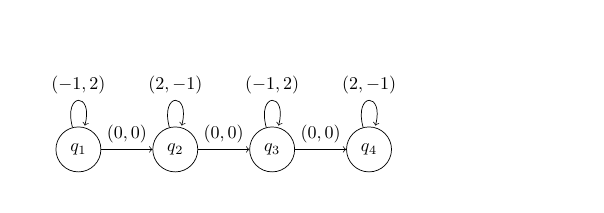
\begin{tikzpicture}[scale=0.25]
\usetikzlibrary{automata, positioning}
\scalebox{0.65}{
\node[state] (q1) {$q_1$};
\node[state, right=of q1] (q2) {$q_2$};
\node[state, right=of q2] (q3) {$q_3$};
\node[state, right=of q3] (q4) {$q_4$};

\path[->] (q1) edge [loop above] node[above] {$(-1,2)$} (q1) edge node[above] {$(0,0)$} (q2); 
\path[->] (q2) edge [loop above] node[above] {$(2,-1)$} (q2) edge node[above] {$(0,0)$} (q3);
\path[->] (q3) edge [loop above] node[above] {$(-1,2)$} (q3) edge node[above] {$(0,0)$} (q4);
\path[->] (q4) edge [loop above] node[above] {$(2,-1)$} (q4);
}
\end{tikzpicture}
\end{minipage}
\begin{minipage}{0.32\textwidth}
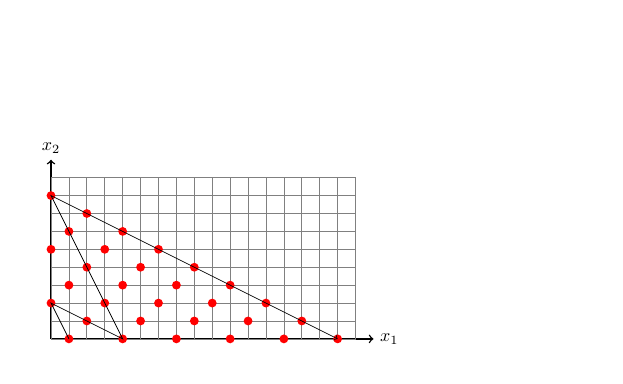
\begin{tikzpicture}[scale=0.35]
\scalebox{0.65}{
\draw[->, thick] (0, 0) -- (18, 0) node[right] {$x_1$};
\draw[->, thick] (0, 0) -- (0, 10) node[above] {$x_2$};

\draw[step=1, gray, thin] (0, 0) grid (17, 9);

\foreach \x in {1,4,7,10,13,16} \fill[red] (\x,0) circle (7pt);
\foreach \x in {2,5,8,11,14} \fill[red] (\x,1) circle (7pt);
\foreach \x in {0,3,6,9,12} \fill[red] (\x,2) circle (7pt);
\foreach \x in {1,4,7,10} \fill[red] (\x,3) circle (7pt);
\foreach \x in {2,5,8} \fill[red] (\x,4) circle (7pt);
\foreach \x in {0,3,6} \fill[red] (\x,5) circle (7pt);
\foreach \x in {1,4} \fill[red] (\x,6) circle (7pt);
\foreach \x in {2} \fill[red] (\x,7) circle (7pt);
\foreach \x in {0} \fill[red] (\x,8) circle (7pt);

\draw[->] (1,0) -- (0,2) -- (2,1) -- (4,0) -- (3,2) -- (2,4) -- (1,6) -- (0,8) -- (2,7) -- (4,6) -- (6,5) -- (8,4) -- (10,3) -- (12,2) -- (14,1) -- (16,0);
}
\end{tikzpicture}
\end{minipage}
\begin{minipage}{0.32\textwidth}
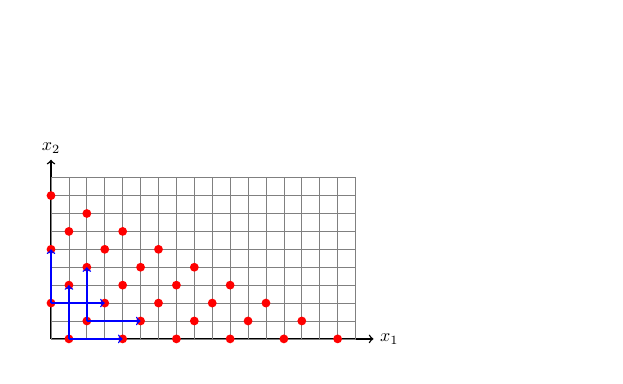
\begin{tikzpicture}[scale=0.35]
\scalebox{0.65}{
\draw[->, thick] (0, 0) -- (18, 0) node[right] {$x_1$};
\draw[->, thick] (0, 0) -- (0, 10) node[above] {$x_2$};

\draw[step=1, gray, thin] (0, 0) grid (17, 9);

\foreach \x in {1,4,7,10,13,16} \fill[red] (\x,0) circle (7pt);
\foreach \x in {2,5,8,11,14} \fill[red] (\x,1) circle (7pt);
\foreach \x in {0,3,6,9,12} \fill[red] (\x,2) circle (7pt);
\foreach \x in {1,4,7,10} \fill[red] (\x,3) circle (7pt);
\foreach \x in {2,5,8} \fill[red] (\x,4) circle (7pt);
\foreach \x in {0,3,6} \fill[red] (\x,5) circle (7pt);
\foreach \x in {1,4} \fill[red] (\x,6) circle (7pt);
\foreach \x in {2} \fill[red] (\x,7) circle (7pt);
\foreach \x in {0} \fill[red] (\x,8) circle (7pt);

\draw[->,blue,thick] (1,0) -- (4,0);
\draw[->,blue,thick] (1,0) -- (1,3);

\draw[->,blue,thick] (2,1) -- (5,1);
\draw[->,blue,thick] (2,1) -- (2,4);

\draw[->,blue,thick] (0,2) -- (3,2);
\draw[->,blue,thick] (0,2) -- (0,5);
}
\end{tikzpicture}
\end{minipage}
\caption{Left: 4-component \dvass $V_2$. 
Middle: the set $\reach_{q_4}(V_2, q_1(1,0))$ and a path $q_1(1,0) \tran q_4(16,0)$.
Right: bases 
%$A = \{(1,0),(2,1),(0,2)\}$ 
and periods 
%$P = \{(0,3),(3,0)\}$
 of an over-approximating semi-linear set $A+P^*$.}
\label{fig:zigzag}
\end{figure}

\begin{example}
For $k\geq 1$, let $V_k$ be a $(2k)$-component \dvass, where each component has just one state $q_i$
and one transition:
$(q_i, (-1,2), q_i)$ for odd $i$, and $(q_i, (2,-1), q_i)$ for even $i$.
Bridge transitions are $(q_i, (0,0), q_{i+1})$.
Figure~\ref{fig:zigzag} shows $V_2$ (left) and 
a path in $V_2$ from $s = q_1(1,0)$ to $t = q_4(16,0)$ together with 
the reachability set $\reach_{q_4}(V_2, s)$ (middle).
In general,
\begin{align} \label{eq:reachk}
X_k := \reach_{q_{2k}}(V_k, s) \ = \ \set{(x_1,x_2) \mid x_1+2x_2 \leq 4^k, \  x_1+2x_2 \equiv 1 \!\! \mod 3}.
\end{align}
Even if the size of the reachability set is 
exponential in $k$, for small $(x_1, x_2)$ it is periodic and the periods are small.
The set $X_k$ can be over-approximated by $A + P^*$ for $A = \set{(1,0),(2,1),(0,2)}$ and $P = \set{(0,3),(3,0)}$
(shown on the right of Figure~\ref{fig:zigzag}), namely for every $k\geq 1$ and $B\in\N$,
the set $X_k$ is \kanapka {$8$} {$B$}. 
For illustration, consider $Y := X_k \cap ((1,0) + P^*)$.
If $(1,0) + P^{\leq B} \subseteq X_k$ then $Y$ is a $B$-approximation
of $(1,0) + P^*$ with $\norm((1,0)), \norm(P) \leq 3 \leq 8$. 
Otherwise, there is some $(v_1, v_2) \in \big((1,0) + P^{\leq B}\big)\setminus X_k$, and
then $B$ is larger than $4^k$:
\[
%8B \geq 2(1 + 3B) \geq 2(v_1 + v_2) \geq v_1 + 2 v_2 > 
4^k < v_1 + 2 v_2 \leq 2(v_1 + v_2) \leq 2(1+3B) \leq 8B.
\]
Therefore by \eqref{eq:reachk}, each $(x_1,x_2) \in Y$ satisfies 
$\norm(x_1,x_2) = x_1 + x_2 \leq x_1 + 2x_2 \leq 4^k < 8B$, and thus
$Y$, seen as a union of singletons, is a union of 
linear sets with norm of base bounded by $8B$ and empty set of periods. 
In both cases, 
$Y$ is \kanapka {$8$} {$B$}. 
%The same intuition stays behind polynomial approximability of \dvass stated in Lemma~\ref{lem:2vass-sandwich}.
\end{example}

\end{document}
